\documentclass[10pt,twocolumn,letterpaper]{article}
%\usepackage[latin1]{inputenc}

%\usepackage{url}
%\usepackage{booktabs}

\usepackage{cvpr}
\usepackage{times}
\usepackage{epsfig}
\usepackage{graphicx}
\usepackage{grffile}
\usepackage{amsmath}
\usepackage{amssymb}
\usepackage{amsmath}
\usepackage{amsfonts}
\usepackage{subfigure}
\usepackage{nonfloat}
\usepackage{url}
\usepackage[colorlinks=true, linkcolor=green, pagebackref]{hyperref}
\usepackage{textcomp} % for textonehalf
%\usepackage{subfig}
%\usepackage{subref}
%\usepackage{booktabs}

\usepackage{wrapfig}
\graphicspath{{imgs/}{data/renders_turn_table/}}

\usepackage{xspace}
\renewcommand*{\eg}{e.g.\@\xspace}
\renewcommand*{\ie}{i.e.\@\xspace}
\newcommand*{\ea}{et al.\@\xspace}
\renewcommand*{\vs}{vs.\@\xspace}
%\renewcommand{\arraystretch}{1.5}

%\cvprfinalcopy % *** Uncomment this line for the final submission

\def\cvprPaperID{1437} % *** Enter the CVPR Paper ID here
\def\httilde{\mbox{\tt\raisebox{-.5ex}{\symbol{126}}}}

% General notation
\newcommand{\prob}{Pr}
\newcommand{\degree}{^{\circ}}
\newcommand{\feat}{\mathbf{x}}

% Image notation
\newcommand{\rgbdimage}{\mathcal{D}}
\newcommand{\intrinsics}{K}
\newcommand{\pixelidx}{\mathbf{s}}
\newcommand{\edgeimidx}{\mathbf{e}}

% Voxel notation
\newcommand{\voxelgrid}{\mathcal{V}}
\newcommand{\voxel}{v}
\newcommand{\voxidx}{i}
\newcommand{\voxelidxs}{m, n, l}

% Point cloud notation
\newcommand{\project}{\mathbf{p}}
\newcommand{\pcloud}{\mathcal{P}}
\newcommand{\point}{\mathbf{p}}
\newcommand{\normal}{\mathbf{n}}
\newcommand{\updir}{\mathbf{u}}

% Transformations
\newcommand{\trans}{T}
\newcommand{\extrinsics}{H}
\newcommand{\voxelgridtoworld}{\trans_{\voxelgrid \rightarrow w}}


\definecolor{red}{rgb}{0.95,0.4,0.4}
\definecolor{blue}{rgb}{0.4,0.4,0.95}
\definecolor{darkred}{rgb}{0.8,0,0}
\definecolor{darkgreen}{rgb}{0,0.5,0}
\definecolor{grey}{rgb}{0.6,0.6,0.6}

\newcommand{\todo}[1]{\textcolor{red}{TODO: #1}}
\newcommand{\note}[1]{\textcolor{blue}{NOTE: #1}}
\newcommand{\status}[1]{\textcolor{blue}{Status: #1}}
\newcommand{\add}[1]{\textcolor{darkgreen}{#1}}
\newcommand{\remove}[1]{\textcolor{grey}{#1}}

\renewcommand{\paragraph}{\vspace{2pt}\noindent\textbf}

%[citecounter=true, style=ieee]
%\usepackage{biblatex}
%\addbibresource{bibtex/strings.bib}
%\addbibresource{bibtex/main.bib}
%\addbibresource{bibtex/crossrefs.bib}
%addbibresource{\jobname.bib}


\title{Structured Prediction of Unobserved Voxels From a Single Depth Image}

%\author{Michael Firman, Gabriel Brostow, Simon Julier \ea}

\begin{document}


\maketitle

\begin{abstract}
	%Building a representation of the geometry of a scene is an essential task for many applications including robotic navigation, scene re-lighting and object manipulation.
	%Most existing works to recover the scene geometry rely on combining multiple views of the scene captured from many different directions or use of \emph{a priori} information about the expected semantic make-up of the scene.
  Building a complete 3D model of a scene is underconstrained given a single camera view.
  To gain a full volumetric model, one typically needs either multiple views, or a single view together with the strong assumption that one has a library of unambiguous training instances that fit the shape of each individual object in the scene.

  We hypothesize that objects of dissimilar semantic classes often share similar shape components, enabling a limited dataset to model the shape of a wide range of objects, and hence estimate the hidden geometry of various scenes.
  Exploring this hypothesis, we have implemented a system that can complete the unobserved geometry of a scene using a library of simple volumetric elements learned from training data.
  Using a novel feature representation, we train a model to map from observed depth values to an estimate of surface shape in the neighborhood of a 3D location.
  Through the prototype, we validate our approach qualitatively and quantitatively on a range of indoor scenes.

\end{abstract}

%%%%%%%%%%%%%%%%%%%%%%%%%%%%%%%%%%%%%%%%%%%%%%%%%%%%%%%%%%%%%%
\section{Introduction}
%\footnote{Potential to add to intro: Psychology: Are humans good at this? Not much evaluation in other work.}
%%%%%%%%%%%%%%%%%%%%%%%%%%%%%%%%%%%%%%%%%%%%%%%%%%%%%%%%%%%%%%


% What is the problem?
We broadly categorize space in our world as being `occupied' and opaque, or `vacant' and transparent.
Depth cameras such as the Microsoft Kinect are able to give an estimate of which regions of a scene are composed of free, vacant space.
However, each pixel in a depth image only makes an estimate of occupancy in front of the first solid surface encountered along that camera ray (Figure \ref{fig:intro}).
The `occlusion phenomenon' prevents any information from being measured about the occupancy of space beyond that first surface.

% Why is it interesting and important?
There are many applications, however, which critically require a complete representation of the world geometry.
When a robot sets out to grasp an unknown object in an unknown scene, a 3D model is required to get there and prevent collision with the object or nearby clutter.
Separately, in photo-editing, the full geometry would enable realistic shadows from a new light source to be automatically added to an image after it has been captured.

% Why is it hard? (E.g., why do naive approaches fail?)
Much computer vision research has been invested in reconstructing a full 3D world model from images of a scene captured from multiple viewpoints, thus coping with the effects of occlusion  (\eg \cite{izadi-uist-2011}).
Instead, we focus on the task of classifying each voxel in a 3D scene as being either `occupied' or `vacant' given just a single depth image from one viewpoint.
%% THERE WILL ALWAYS BE HOLES, EVEN WITH KINFU %%

\newcommand{\introsubwidth}{0.48\columnwidth}
\begin{figure}[!t]
    \centering
    \subfigure[Voxel world model]{%
        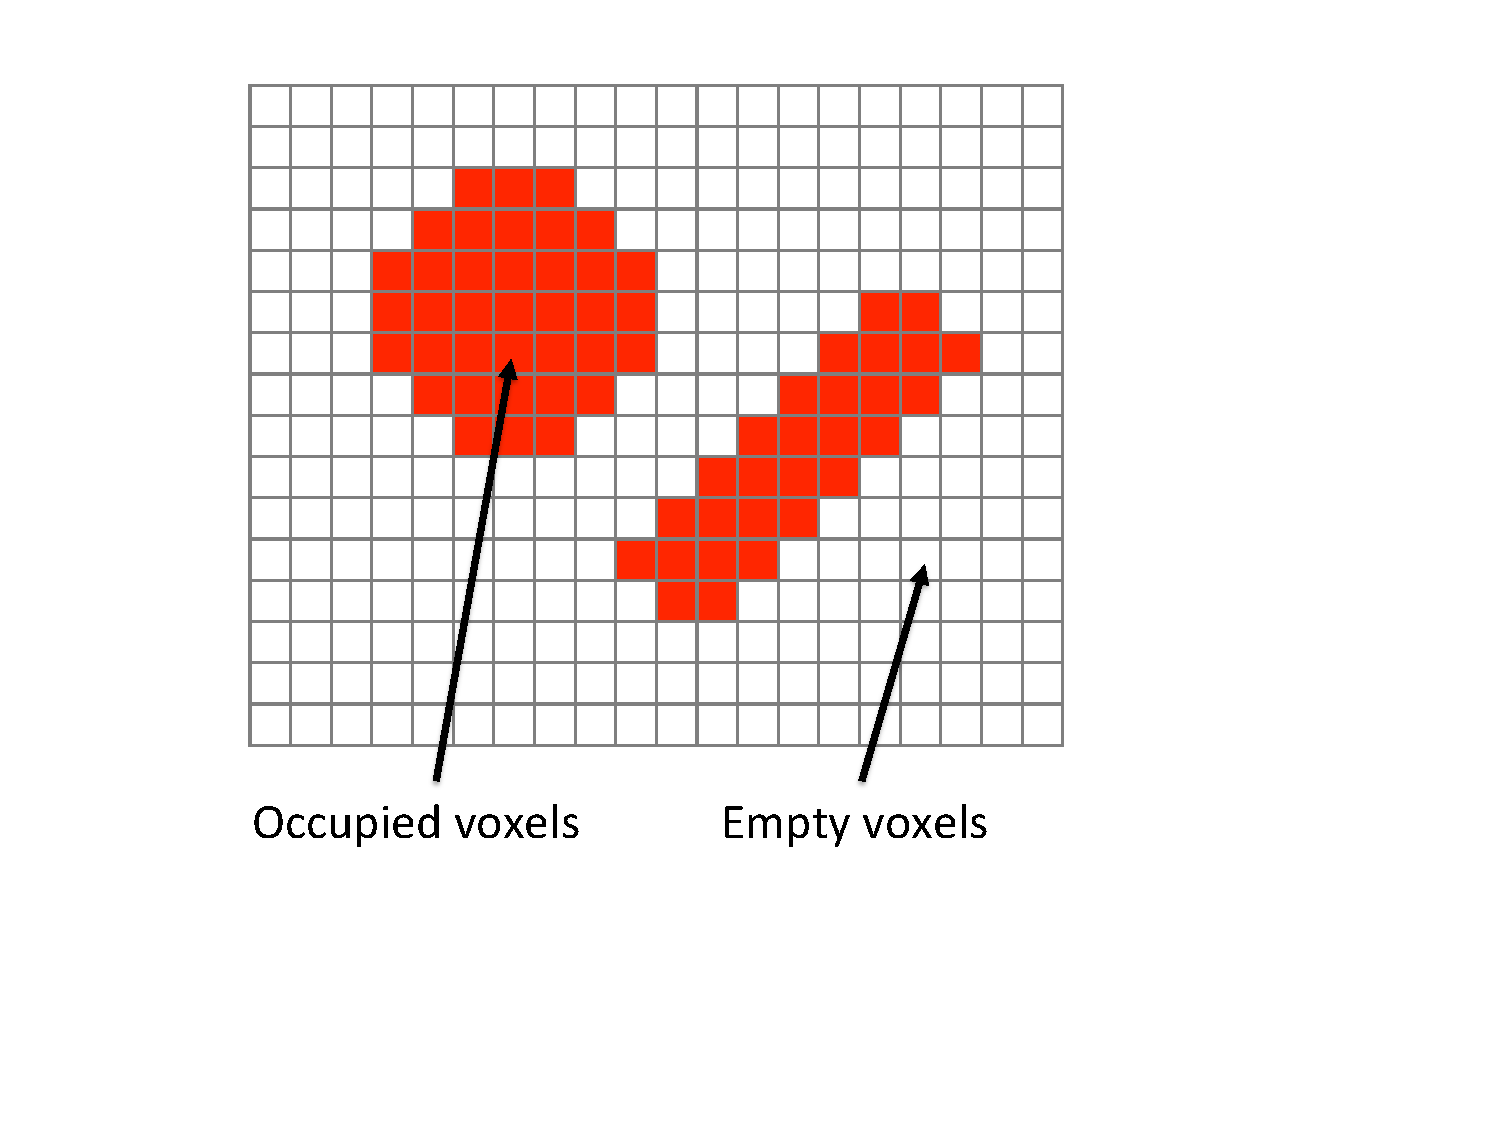
\includegraphics[width=\introsubwidth, clip=true, trim=110 105 205 30]{fig_1}}
        \hfill
    \subfigure[Depth rendering of world]{%
        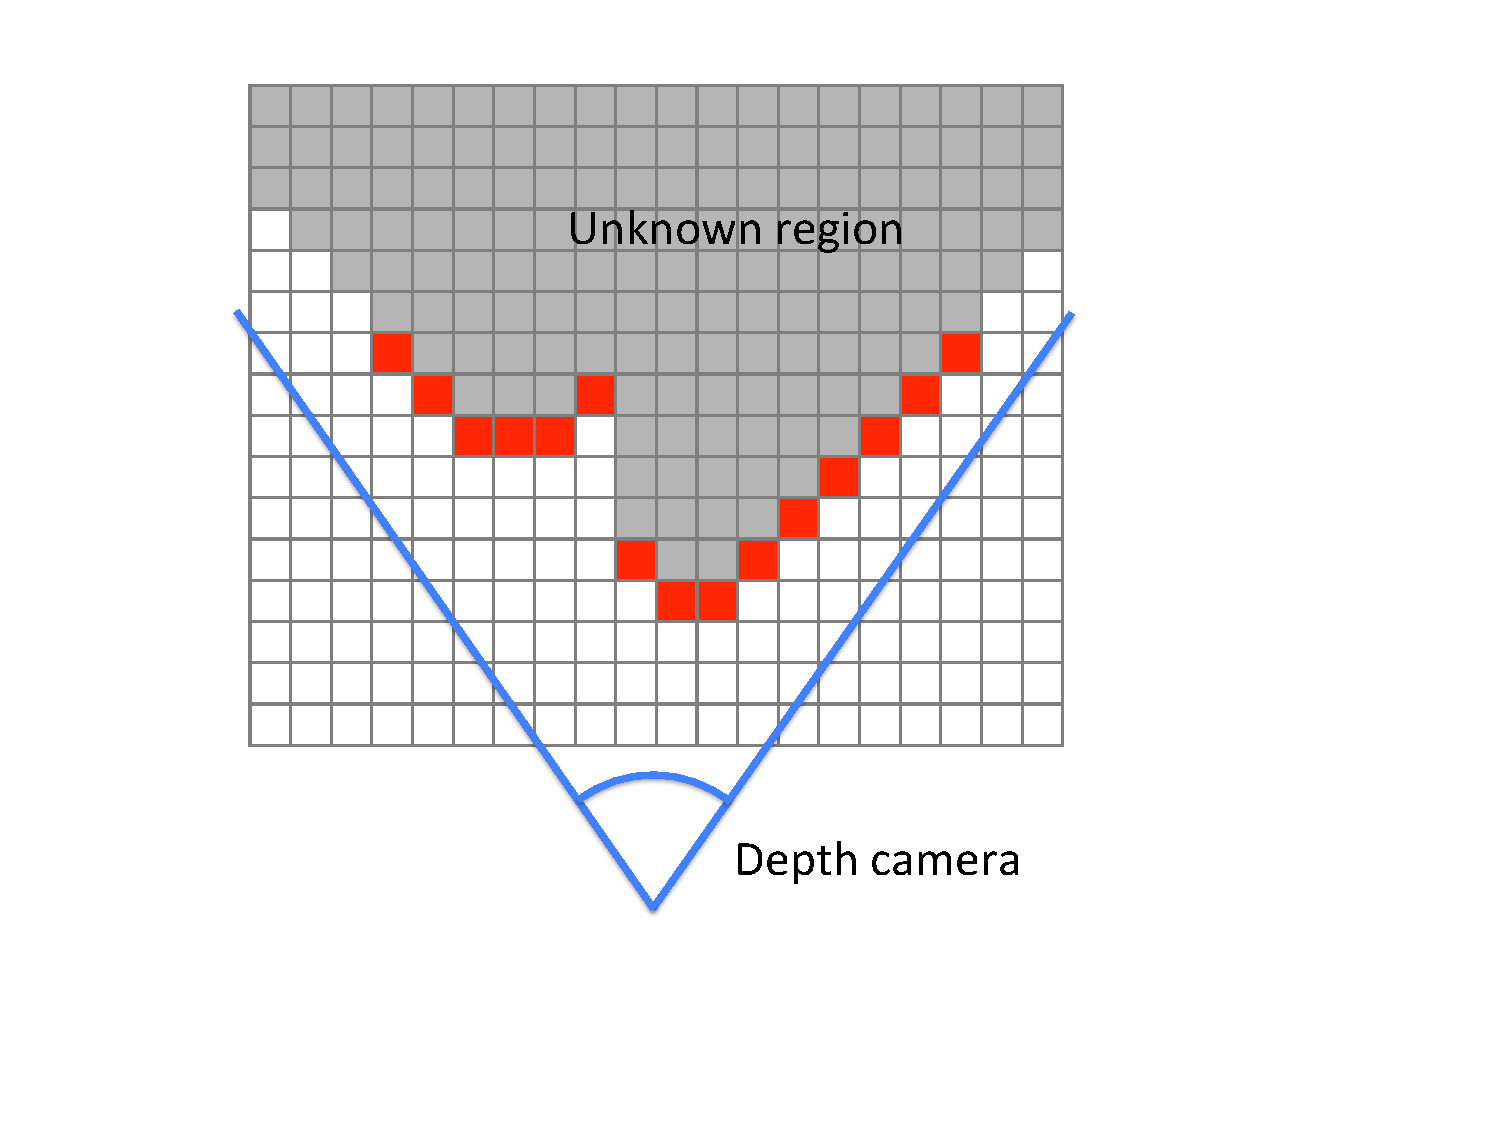
\includegraphics[width=\introsubwidth, clip=true, trim=110 105 205 30]{fig_1b}}
    \caption{
    We model our world as a grid of voxels, each of which is either occupied or empty (vacant).
    An overhead view of a coarse 2D representation of this is shown in (a).
    When observed by a depth camera, only the first voxel along each ray is seen.
    This leaves a region of unknown occupancy extending beyond the depth surface (b).
    The aim of our algorithm is to predict the state of the voxels in this unknown region.}%
    \label{fig:intro}
\end{figure}

%%%%%%%%%%%%%%%%%%%%%%%%%%%%%%%%%%%%%%%%%%%%%%%%%%%%%%%%%%%%%%
\subsection{Our approach and contributions}
%%%%%%%%%%%%%%%%%%%%%%%%%%%%%%%%%%%%%%%%%%%%%%%%%%%%%%%%%%%%%%

Given a single depth image, our system predicts whether each voxel in the scene is occupied by a solid impermeable object, or free and empty.
In effect, we strive to predict the voxelized output of KinectFusion \cite{izadi-uist-2011}, but having test-time input of only a single view of the scene instead of multiple views.

We achieve this by learning a mapping from local and novel semi-regional features on a depth image to a structured prediction of geometry in the region of a query point, using a general-purpose collection of training objects and scenes.
We take inspiration from recent work which has segmented objects from images using silhouettes learned from different object classes \cite{kim-eccv-2012}.
This work showed that shape can transcend class categories, enabling shape predictions to be made regardless of the accuracy of semantic classifiers.
Because we care about shape, independently of semantic understanding, we are free to use training objects which differ from the objects being modeled in the scene.

The key contributions that underpin our novel depth image to voxel geometry framework are:
\begin{itemize}
\item \emph{Voxlets}, a representation of multi-voxel geometry in the region of a point in a scene.
We use a Random Forest to learn a mapping from a point in a depth image to a structured prediction of geometry in the region near the point.
\item A novel feature representation for a point in a depth image, which captures both local and region-level shape for a single point in a depth image.
\end{itemize}


%%%%%%%%%%%%%%%%%%%%%%%%%%%%%%%%%%%%%%%%%%%%%%%%%%%%%%%%%%%%%%
\section{Related work}
%%%%%%%%%%%%%%%%%%%%%%%%%%%%%%%%%%%%%%%%%%%%%%%%%%%%%%%%%%%%%%

%Most prior work in the area of completing missing data can be categorized according to its application domain (\eg meshes \cite{schnabel-eurographics-2009, ju-cst-2009}, 2D images \cite{gupta-cvpr-2011} or depth images \cite{shen-tog-2012}).


%\subsection{Taxonomy of related works}
Previous works on completing unknown regions of visual data can be categorized against several different criteria.
Some of these are given here, and we italicize the categories into which our approach falls.

Works can be classed according to their application domain, such as operating on meshes \cite{harary-tog-2013, schnabel-eurographics-2009}, 2D images \cite{gupta-cvpr-2011} or in \emph{voxel space} \cite{kim-iccv-2013}.
Some works make use of highly specialist hardware to capture images \eg \cite{velten-nature-2012}, while we use \emph{hardware available to consumers}.
Some approaches only aim to get a result that looks plausible to a human, while we strive for \emph{accuracy in comparison to the ground truth}.
In comparison to works which use heuristics, we make use of \emph{training data}.
Such supervised approaches can be further classed according to whether the data used come from within the same image (\eg symmetry \cite{kroemer-humanoids-2012}) or from a \emph{database of training data}.

We now outline some of these previous approaches in more detail, and compare them to our approach.


%%%%%%%%%%%%%%%%%%%%%%%%%%%%%%%%%%%%%%%%
\paragraph{Fitting 3D models}
If prior knowledge is available about the objects present in the scene, in the form of 3D models, then an instance-level model can be fitted to a 3D scene.
This gives a good recovery of missing geometry of that object \cite{hinterstoisser-accv-2012, drost-3dimpvt-2012}.
Some works focus on the broader problem where an exact match is not present in the training set.
Shen \ea \cite{shen-tog-2012} complete the missing regions of a single object using an assembly of parts from several different models in a CAD database.
Cocias \ea \cite{cocias-cgvcv-2013} directly deform a mesh to fit to a point cloud, while Prisacariu and Reid \cite{prisacariu-iccv-2011} fit a class-level manifold model to the image data.

%Collecting training data for this is laborious and costly, and currently there do not exist enough 3D models suitable for accurately completing most real-world scenes.
All these methods, however, rely on the availability of some form of specific prior model, and this completion method relies on an accurate detector to find and classify each object in the scene.
In our approach, we set out to get as much shape information as possible \emph{without semantics}, thus remaining free of its associated machinery and limitations.



%%%%%%%%%%%%%%%%%%%%%%%%%%%%%%%%%%%%%%%%
\paragraph{Symmetry}
Where one can accurately detect symmetry, it can be leveraged to complete some types of objects (\eg \cite{law-cviu-2010, thrun-iccv-2005, kroemer-humanoids-2012}).
However, using symmetry for object completion is brittle.
If symmetry cannot be detected at all, then no prediction can be made.
This is the case for example when viewing a cuboid end-on.
%Our algorithm allows for a reasonable prediction to be made even when no axes of symmetry can be detected.


%%%%%%%%%%%%%%%%%%%%%%%%%%%%%%%%%%%%%%%%
\paragraph{Voxel space reasoning}
The two algorithms which bear the most similarity to ours both make predictions of full scene geometry from a single depth image.

Kim \ea \cite{kim-iccv-2013} use a CRF model over a voxel representation of a scene to simultaneously predict occupancy, visibility and semantic labeling of voxels from an RGBD image.
For training, they use manually labeled top-down views of the scene.
Their final labelings are found from graph cuts over the CRF.
They primarily model the probability of a voxel being occupied as a Gaussian centered on the first observed voxel along a camera ray.
However, high-order-terms in the CRF are used to enforce planar structures and for `objects' to remain contiguous.

Like \cite{kim-iccv-2013},  Zheng \ea \cite{zheng-cvpr-2013} go from a single depth image to a voxel representation of a scene.
Their core algorithm consists of two parts.
Firstly they complete missing voxels by extruding visible points in the detected Manhattan World directions of the scene.
This part bears resemblance to a similar method used for completions by \cite{kroemer-humanoids-2012}.
Secondly, they use physics-based reasoning to fill in missing data to ensure connectedness and stability.
The physics-based reasoning is clearly useful in complex scenes where, for example, a table leg may be occluded.
However the voxel completion by extrusion is limited by the Manhattan World assumption, and the extent of visible voxels in the scene.

In contrast to these methods, we are able to make \emph{structured} predictions in 3D space, thus being able to make predictions about shape learned directly from training data.
%we are able to complete objects where the points making up the objects are hard to see.}


%%%%%%%%%%%%%%%%%%%%%%%%%%%%%%%%%%%%%%%%
\paragraph{Surface completion}
Silberman \ea \cite{silberman-eccv-2014} tackle the completion of an incomplete multi-view reconstruction as a surface completion problem.
By detecting planes, they can complete their contours in a 2D projection using a novel CRF method.
This method, however, relies both on a piecewise-planar scene, and on beginning with an almost-complete scan as input.

Davis \ea \cite{davis-3dpvt-2002} complete surfaces by operating directly on the \emph{signed distance field}, the zero level-set of which defines the surface location. They diffuse the signed distance field across holes in the mesh to fill in the gaps.
\cite{harary-tog-2013} use a data-driven approach, finding matches in the mesh to the missing region.

All of these completion methods are only suitable where the set of missing data is small relative to the size of the observed data.
In our case, we are completing the geometry of an unknown surface which is typically at least as large as the observed surface.


%%%%%%%%%%%%%%%%%%%%%%%%%%%%%%%%%%%%%%%%
\paragraph{Image completion and super-resolution}
Image completion works such as \cite{hays-siggraph-2007, criminisi-cvpr-2003}
typically use region-based data-driven approaches as it is very difficult to form true generative models over image appearance.
For example, \cite{hays-siggraph-2007} look up possible completion regions in a large database of similar images, while \cite{criminisi-cvpr-2003} in-paint by selecting and combining multiple plausible patches from other regions of the input image.
This differs from our task, as image completion typically aims for a visually plausible output, irrespective of the accuracy compared to ground truth.
Similar to image \emph{completion} is image \emph{super-resolution}, \eg \cite{macaodha-eccv-2012}.
This, like our problem, is ill-posed and relies on the repeatability and predictability of the world in order to improve the local geometry of an image.
Our problem differs from that of super-resolution because we make predictions about the state of the world outside of the region directly observable by the camera.


%%%%%%%%%%%%%%%%%%%%%%%%%%%%%%%%%%%%%%%%
\paragraph{Using 3D primitives for recognition}
`Geons' are proposed by \cite{bieberman-rbc-1987} as a set of 3D primitives such as cylinders and cuboids used by humans in their recognition of object shapes.
While in theory, geons could be used by computers  as features to describe natural objects, in practice, this was found to be challenging \cite{dickinson-iavc-1997} due to their ``idealized nature'', requirement for part segmentation, labeling errors, and the coarseness of features used to extract geons in the first place.
%Besl - hand-defined

However, fitting bounding boxes has recently become a popular method to explain the arrangement of objects in a scene.
Recent work has successfully incorporated high-level information such as gravity and stability
 \cite{shao-siggraphasia-2014, jia-cvpr-2013}, and made use of training data to accurately detect bounding box locations \cite{hedau-cvpr-2012}.
Gupta \ea \cite{gupta-cvpr-2011} estimate voxel occupancy from a 2D image, which is regularized using cuboid bounding box hypotheses.
The obvious problem with bounding box style methods is that they can only give coarse shape information, which is not suitable for many applications of geometry completion.

In our work, we make use of 3D primitives.
However, unlike geons which are fixed in shape, we learn a distribution of shapes from training data.
We are also able to make more fine-grained predictions than bounding boxes.



\begin{figure*}
    \subfigure[Query point]{%
        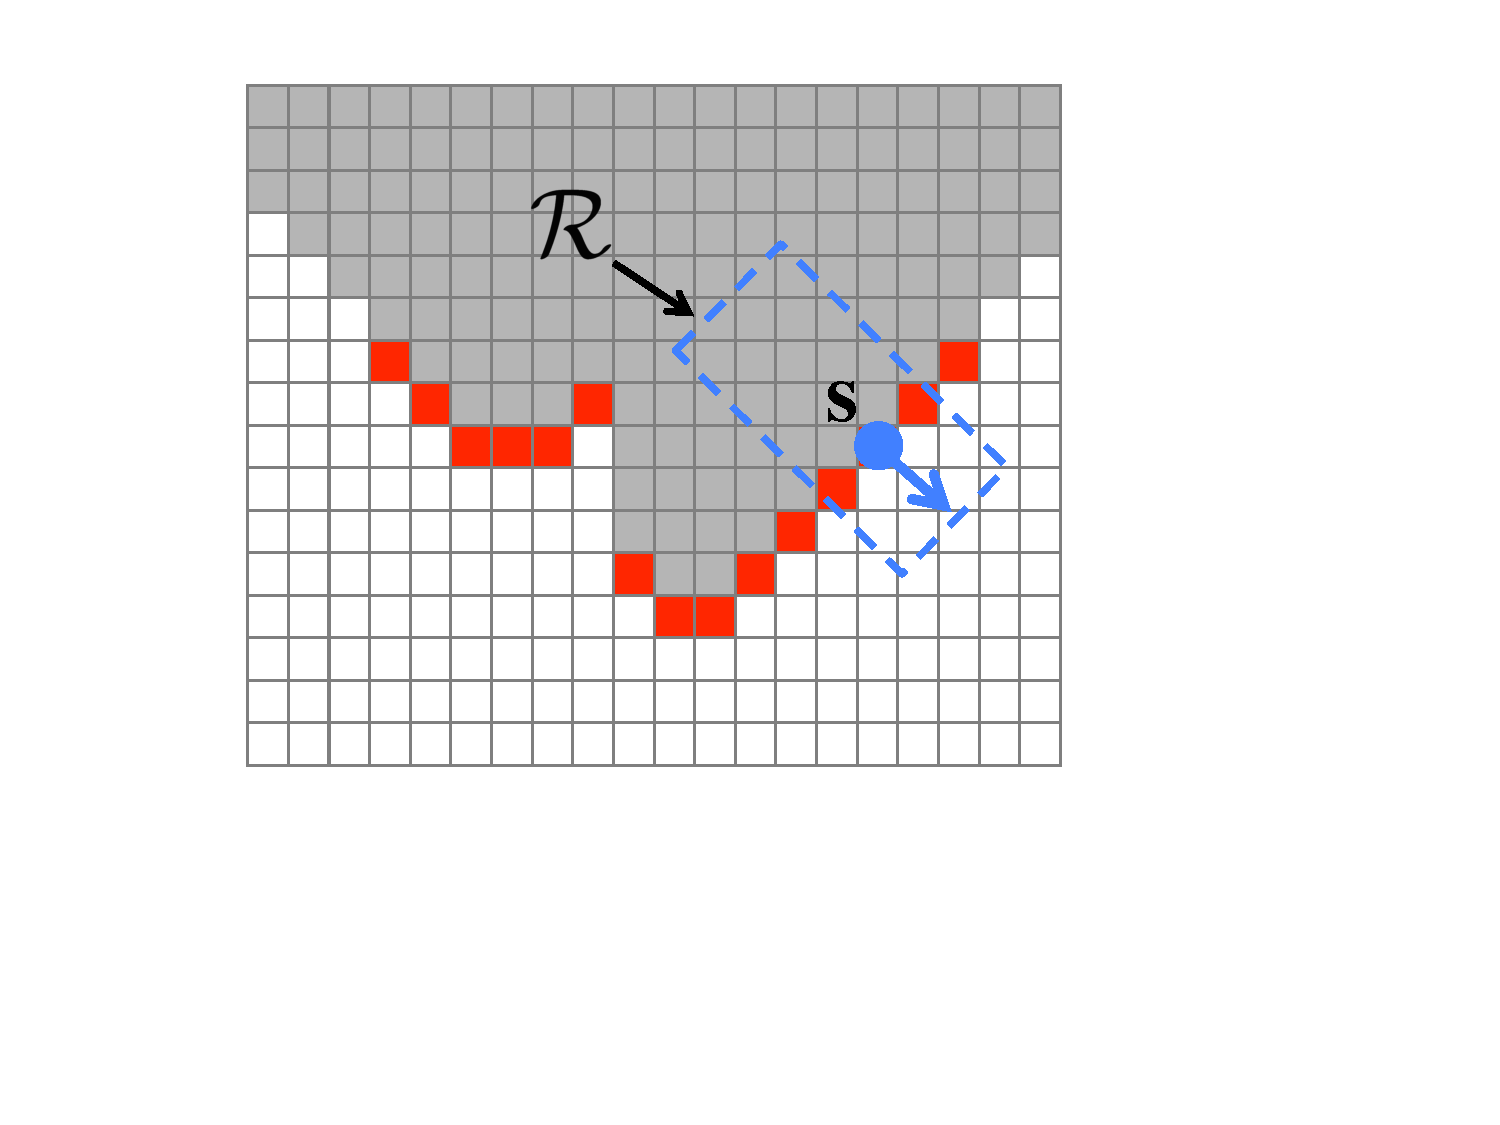
\includegraphics[width=0.5\columnwidth, clip=true, trim=110 170 205 30, page=1]{overview_image}\label{subfig:voxregion}}
        \hfill
    \subfigure[Forest prediction]{%
        \includegraphics[width=0.45\columnwidth, clip=true, trim=80 170 265 30, page=2]{overview_image}\label{subfig:forest_overview}}
        \hfill
    \subfigure[Insertion into voxel grid]{%
        \includegraphics[width=0.5\columnwidth, clip=true, trim=110 170 205 30, page=3]{overview_image}\label{subfig:alignment}}
        \hfill
      \subfigure[Multiple predictions]{%
        \includegraphics[width=0.5\columnwidth, clip=true, trim=110 170 205 30, page=4]{overview_image}}
    \caption{\textbf{Overview of our algorithm, shown diagrammatically in a 2D representation.}
    (a) At test time, we define a cuboid region of voxels $\mathcal{R}$ around a query point $\pixelidx$.
    This cuboid is aligned with the normal at $\pixelidx$.
    (b) A feature representation $\mathbf{x}(\mathbf{s})$ is put through our pre-trained Random Forest.
    The forest makes a prediction for the values of each of the voxels in $\mathcal{R}$.
    (c) This prediction is transformed into the scene and used to update the values of the voxels.
    (d) The aggregation of multiple such predictions forms our final prediction of the TSDF, which can be converted to voxel occupancy or a surface representation.
    }%
    \label{fig:overview}
\end{figure*}
%%%%%%%%%%%%%%%%%%%%%%%%%%%%%%%%%%%%%%%%
\paragraph{Structured learning for vision}
\emph{Structured learning} has become a popular method for some computer vision tasks.
As with standard supervised learning, structured learning finds a mapping from a feature space to a label space.
In contrast to a traditional one-dimensional label space, however, a structured label space is \emph{multidimensional}.
Feature space is typically limited to a local descriptor of the image, while the label space may be surface normals \cite{fouhey-iccv-2013}, human poses \cite{bourdev-iccv-2009}, or semantic labels.
This family of works provides inspiration for our approach.

%A question that arises is: How to form the set of primitives?
There are many different ways of finding the mapping from feature to structured label space.
For example, \cite{bourdev-iccv-2009} cluster human poses, while \cite{fouhey-iccv-2013} use an SVM-like formulation to find primitives which are both discriminative in feature space and informative in label space.

In our work, we make use of Random Forests \cite{breiman-ml-2001}.
Originally proposed for regression and then single-label classification problems, they have since been adapted to make structured predictions for tasks such as semantic labelling \cite{kontschieder-iccv-2011} and edge detection \cite{dollar-iccv-2013}.
Structured prediction can make faster and more regularized predictions than a single dimensional predictor.
In our case, we benefit from a structured prediction as we are able to make predictions beyond the location of the input data point.

%One example of this is work on edge detection, where an input image patch is mapped to a prediction of the edges in the region of the patch
% \begin{quote}
% Voxel occupancy is one approach for reconstructing the 3-dimensional shape of an object from multiple views. In voxel occupancy, the task is to produce a binary labeling of a set of voxels, that determines which voxels are filled and which are empty.
% \cite{snow-cvpr-2000}
% \end{quote}


% %%%%%%%%%%%%%%%%%%%%%%%%%%%%%%%%%%%%%%%%%%%%%%%%%%%%%%%%%%%%%%%%%%%%%%%%%%%%%%%%
\section{Approach formulation}
% %%%%%%%%%%%%%%%%%%%%%%%%%%%%%%%%%%%%%%%%%%%%%%%%%%%%%%%%%%%%%%%%%%%%%%%%%%%%%%%%


We model the geometry of a scene as a regular grid of voxels $\voxelgrid = \{\voxel_\voxidx\}$.
Following works such as \cite{izadi-uist-2011, prisacariu-iccv-2011}, each $\voxel_\voxidx \in [-d_{\max}, d_{\max}]$ represents the \emph{truncated signed distance function} (TSDF) of the surface of the scene.
Each $|\voxel_\voxidx|$ gives the distance from $\voxel_\voxidx$ to the nearest surface, truncated to a maximum value of $d_{\max}$, which is a parameter.
$\voxel_\voxidx$ is negative if voxel $\voxidx$ is inside solid opaque matter, and positive if it is in free space.
The zero level-set of $\voxelgrid$ therefore represents the surface.

\newcommand{\voxregion}{\mathcal{R}}

Our system maps a point $\pixelidx$ on an input depth image $\rgbdimage$ to a prediction of the TSDF in a set of voxels in the neighborhood of $\pixelidx_p$, which we use to denote the 3D reprojection of $\pixelidx$.
The aggregation of multiple such predictions gives our final TSDF prediction for the scene.

%$\project(\pixelidx)$, where $\project(\pixelidx)$ is the 3D location of $\pixelidx$ in world space.

%\paragraph{Voxel grid alignment}
%We make our predictions in a voxel grid aligned with world coordinates.
%In practice this means that the z direction of the voxel grid is aligned with the up direction of the world space.
%We do not make any Manhattan World assumptions so are free to position the voxel grid at any orientation about the z-axis.


\paragraph{Support regions}
The \emph{support region} $\voxregion \subset \voxelgrid$ is a set of voxels in the neighborhood of $\pixelidx_p$ for which our model can make a prediction of the TSDF.
Each $\voxregion$ is a fixed-size cuboid of voxels, whose x-axis aligned with the normal direction at $\pixelidx$ (Figure \ref{subfig:voxregion}).

In a 2D world, the location of $\pixelidx$ and the direction of its normal can unambiguously define the location and orientation of $\voxregion$.
However, in 3D there is a degree of freedom unconstrained as the rotation of the cuboid about the axis of the normal is unspecified.
We resolve this by aligning the cuboid such that its z direction is coincident with the world z-axis, \ie the `up' direction of the scene.
The top and bottom face of each cuboid region $\voxregion$ is therefore parallel with the world's ground plane.

%The normal at $\pixelidx$ is used to constrain the degree of freedom around the z-axis.
%\todo{Figure for this!}
%The cuboid is then rotated about the z-axis so that its y-axis is perpendicular to the normal at $\project(\pixelidx)$.

% \remove{
% Each $\voxregion$ is aligned with the coordinate system
% \begin{equation}
%   \Lambda =
%   \left( \begin{array}{ccc}
%   \updir \times \normal \,\, / \,\,  \| \updir \times \normal \| \\
%   \updir \times (\updir \times \normal) \,\,  / \,\,  \| \updir \times (\updir \times \normal) \|  \\
%   \updir
%   \end{array}\right),
%   % \qquad
%   %(\mathbf{v})_{u} := \mathbf{v} / \| \mathbf{v} \|,
% \end{equation}
% where $\normal$ is the normal at $\point$ and $\updir$ is the `up' direction of the scene (\ie pointing directly away from the direction of gravity).

%We examine each $\feat(\pixelidx)$ from $\rgbdimage$ in turn.

\paragraph{Making a single prediction}
At test time, we map a pixel $\pixelidx$ to a feature representation $\feat(\pixelidx)$, as described in Section \ref{sec:features}.
Using a structured Random Forest, we can make a prediction of the geometry inside of $\voxregion$.
We call this prediction of geometry a \emph{voxlet}.
The voxlet, which comes out of the forest in canonical alignment, is then transformed from its local coordinate system into world space to fill the voxels in $\voxregion$.

The accumulation of multiple such predictions forms our final prediction of our TSDF.
This can then be converted to a prediction of surface geometry, described in Section \ref{sec:combining}.

%This transformation is the rotation $\Lambda$ followed by the translation $\mathbf{p}(\mathbf{\pixelidx}) - C(\mathcal{S})$, where $\mathbf{p}(\mathbf{\pixelidx})$ is the projection of $\pixelidx$ into world space, and $C(\mathcal{S})$ is the center of the voxlet.
%\note{This notation and explanation is a bit of a mess --- suggestions welcome! Also need to reference the figure in the text. Figure will ultimately be split into (a), (b) etc to make this easier.}


\paragraph{Training}
At training time, we similarly define a region $\voxregion$ around each point $\pixelidx$, again of a fixed size.
In this case, the ground truth values of $\voxelgrid$ and hence $\voxregion$ are known.
We use these ground truth TSDF values, together with $\mathbf{x}(\pixelidx)$, to train a Random Forest, as explained in  Section \ref{sec:forest_train}.


% \newcommand{\preprocesssubwidth}{0.41\columnwidth}
% \begin{figure*}[tb]
%     \centering
%     \subfigure[RGB image]{%
%         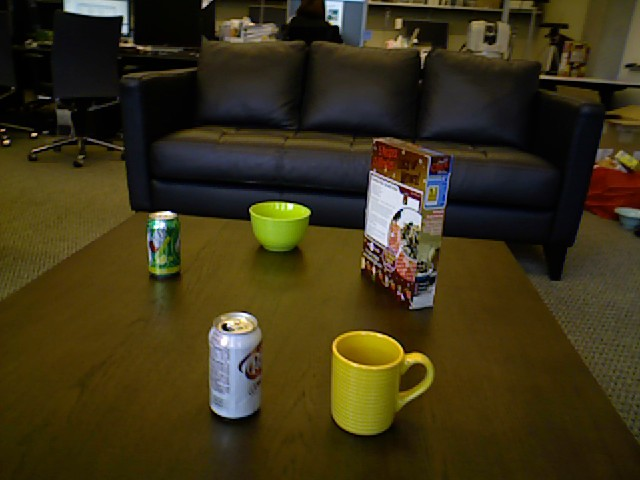
\includegraphics[width=\preprocesssubwidth]{preprocess_a}}
%         \hfill
%     \subfigure[Raw depth image]{%
%         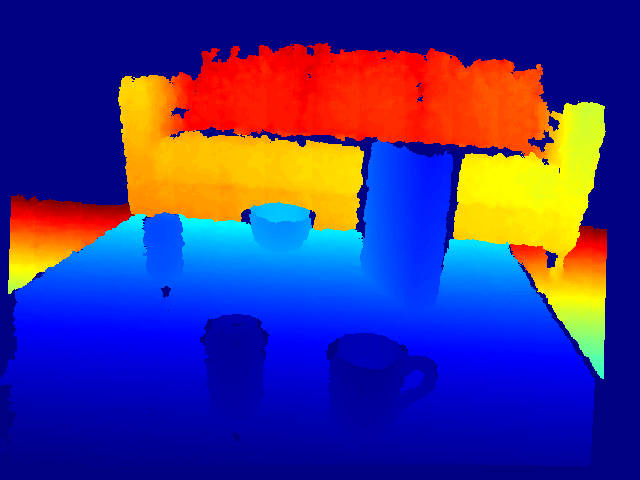
\includegraphics[width=\preprocesssubwidth]{preprocess_b}}
%         \hfill
%     \subfigure[Smoothed depth]{%
%         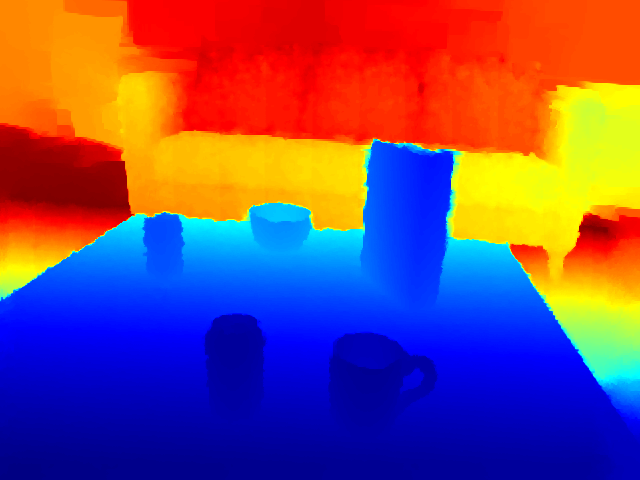
\includegraphics[width=\preprocesssubwidth]{preprocess_c}}
%         \hfill
%     \subfigure[Structured edges]{%
%         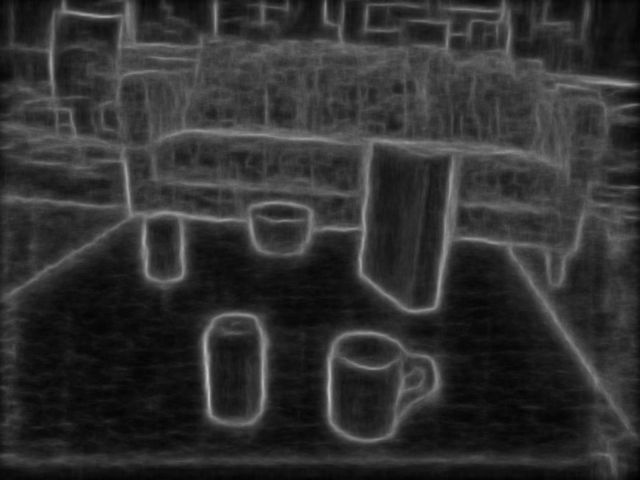
\includegraphics[width=\preprocesssubwidth]{preprocess_d}\label{subfig:structedge}}
%         \hfill
%     \subfigure[Binary edge map]{%
%         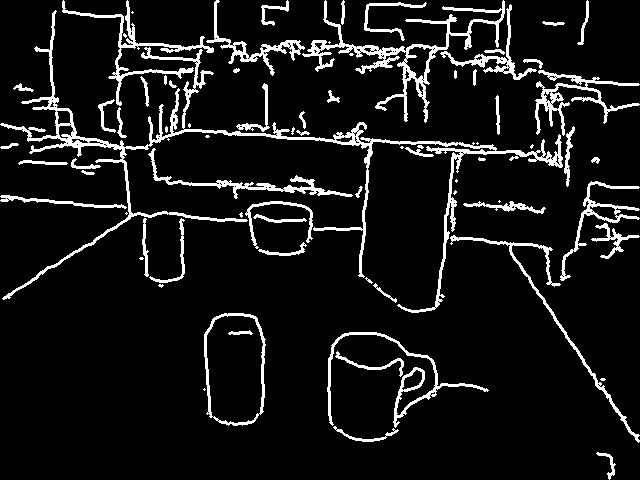
\includegraphics[width=\preprocesssubwidth]{preprocess_e}\label{subfig:binaryedge}}
%     \caption{
%     \todo{Combine this image and the spider image explanation. I can do this on Friday.}
%     The depth image preprocessing pipeline.
%     The noisy depth image (b) is smoothed, and missing data is filled (c).
%     This makes use of the RGB image in the cross-bilateral filtering, where we use the implementation provided by \cite{silberman-eccv-2012}.
%     We then use the structured edge detection model from \cite{dollar-iccv-2013} to compute a real-valued edge map (d) for the image, which is finally binarized (e) using the Canny edge hysteresis method \cite{canny-pami-1986}.
%     }%
%     \label{fig:preprocessing}
% \end{figure*}


%%%%%%%%%%%%%%%%%%%%%%%%%%%%%%%%%%%%%%%%%%%%%%%%%%%%%%%%%%%%%%%%%%%%%%%%%%%%%%%%%
\section{Feature representation}
\label{sec:features}
%%%%%%%%%%%%%%%%%%%%%%%%%%%%%%%%%%%%%%%%%%%%%%%%%%%%%%%%%%%%%%%%%%%%%%%%%%%%%%%%%

\newcommand{\scalfeat}{x}

%Our feature representation maps a pixel location $\pixelidx = (u, v)$ to a feature $\feat(\pixelidx)$, which represents the geometry around the point.
Our feature representation $\feat(\pixelidx)$ at location $\pixelidx$ in the input depth image $\rgbdimage$  describes aspects of its neighborhood.
We use local and regional features extracted from the depth image.
The Random Forest--based model weights feature space to make structured predictions of the truncated signed distance function in the surrounding region.
%This is used in our classifier to map from a single point to a prediction of voxel occupancy in the surrounding region.
% $\feat(\pixelidx) = [\feat_\text{off}(\pixelidx), \feat_\text{spider}(\pixelidx)]$

$\feat(\pixelidx)$ is composed of two parts.
The \emph{offset} feature captures the shape of the depth surface in the immediate neighborhood of $\pixelidx$, and is made up of several local depth comparisons.
The \emph{spider} feature captures the size and shape of the region in the 2D image in which $\pixelidx$ resides.
%, together with the position of $\pixelidx$ in that region.
%\footnote{The names of our features are taken from the shapes they produce in image space (Figure \ref{fig:features}).}.
%$\feat_\text{off}(\pixelidx)$
%$\feat_s(\pixelidx)$


\subsection{Offset feature}
%\pagedepth\maxdimen
\begin{wrapfigure}[10]{r}{0.35\columnwidth}
  \vspace{-20pt}
  \centering
    \includegraphics[width=0.35\columnwidth, clip=true, trim=130 210 340 80, page=9]{spider_cobweb}
    \vspace{-10pt}
  \caption{}%The offset feature}
    \label{fig:offset_feature}
\end{wrapfigure}
The `offset feature' $\scalfeat_\text{off}$ is a simple pairwise feature, used with success in recent work such as \cite{shotton-cvpr-2011}, capturing the surface shape in the immediate neighborhood of pixel $\pixelidx$.
The feature computes the difference between the depth from the camera at $\pixelidx$ and the depth at a predetermined offset $\Delta$ (Figure \ref{fig:offset_feature}). We define
\begin{align}
\scalfeat_\text{off} (\pixelidx, \psi, t) &= \rgbdimage(\pixelidx) - \rgbdimage(\pixelidx + \Delta), \, \text{where} \\
\Delta &= M(t) (\sin(\psi), \cos(\psi)).
\end{align}
Here $M(t) = (t\cdotp f)/\rgbdimage(\pixelidx)$ uses the focal length $f$ to map a distance in world space to a pixel offset.

For a single point $\pixelidx$ we compute $\scalfeat_\text{off} (\pixelidx, \psi, t)$ for a range of different values of $\psi$ and $t$, and concatenate all the values into a feature vector $\feat_{\text{off}}$.
For our experiments we use $\psi, \,\, t \in \{0\degree, 45\degree, \ldots, 315\degree\} \times \{0.02m, 0.04m, 0.06m, 0.08m\}$.
$\feat_{\text{off}}$ is therefore 24-dimensional.
%The pattern of our extracted $\pixelidx + \Delta$ values can be seen in figure \ref{subfig:cobweb}.

%\begin{align}
%F_o (\pixelidx) &= [f_o (\pixelidx, \psi, t) \, :   \psi \in \Psi, t \in \mathcal{T}].
%\end{align}
%\Delta &= M(t) (\sin(\psi), \cos(\psi)).
                %& t \in \{0.02m, 0.04m, 0.06m, 0.08m\}.

%The final feature is then composed of $\Phi(\pixelidx, \psi, t)$ evaluated over a range of values of $\psi$ and $t$.
%For our experiments, we compute the cobweb feature for all combinations of $\psi = [0\degree, 45\degree, \ldots, 315\degree]$ and $t = [0.02m, 0.04m, 0.06m, 0.08m]$.


  %\end{center}
  %\begin{center}
%In our experiments the final feature is then composed of
% as
%\begin{align}
%\feat_c(\pixelidx) &= [\Phi(\pixelidx, \psi, t): \psi = [0\degree, 45\degree, \ldots, 315\degree], t = [0.%02m, 0.04m, 0.06m, 0.08m].
%\end{align}

%a &= \left\lfloor u + M(t)  \sin(\psi) \right\rceil \\
%b &= \left\lfloor v + M(t)  \cos(\psi) \right\rceil

% over a range of values of
%Note also: ``If an offset pixel lies on the background or outside the bounds of the image, the depth probe dI (x0) is given a large positive constant value''.

\newcommand{\pointthreed}{\pixelidx_p}
\newcommand{\edgethreed}{\edgeimidx_p}
\newcommand{\spiderfeat}{s}
\newcommand{\gline}{\mathbf{l}}


\newcommand{\subwidth}{0.32\columnwidth}
\begin{figure}
    \centering
    %\subfigure[Query point]{%
    %    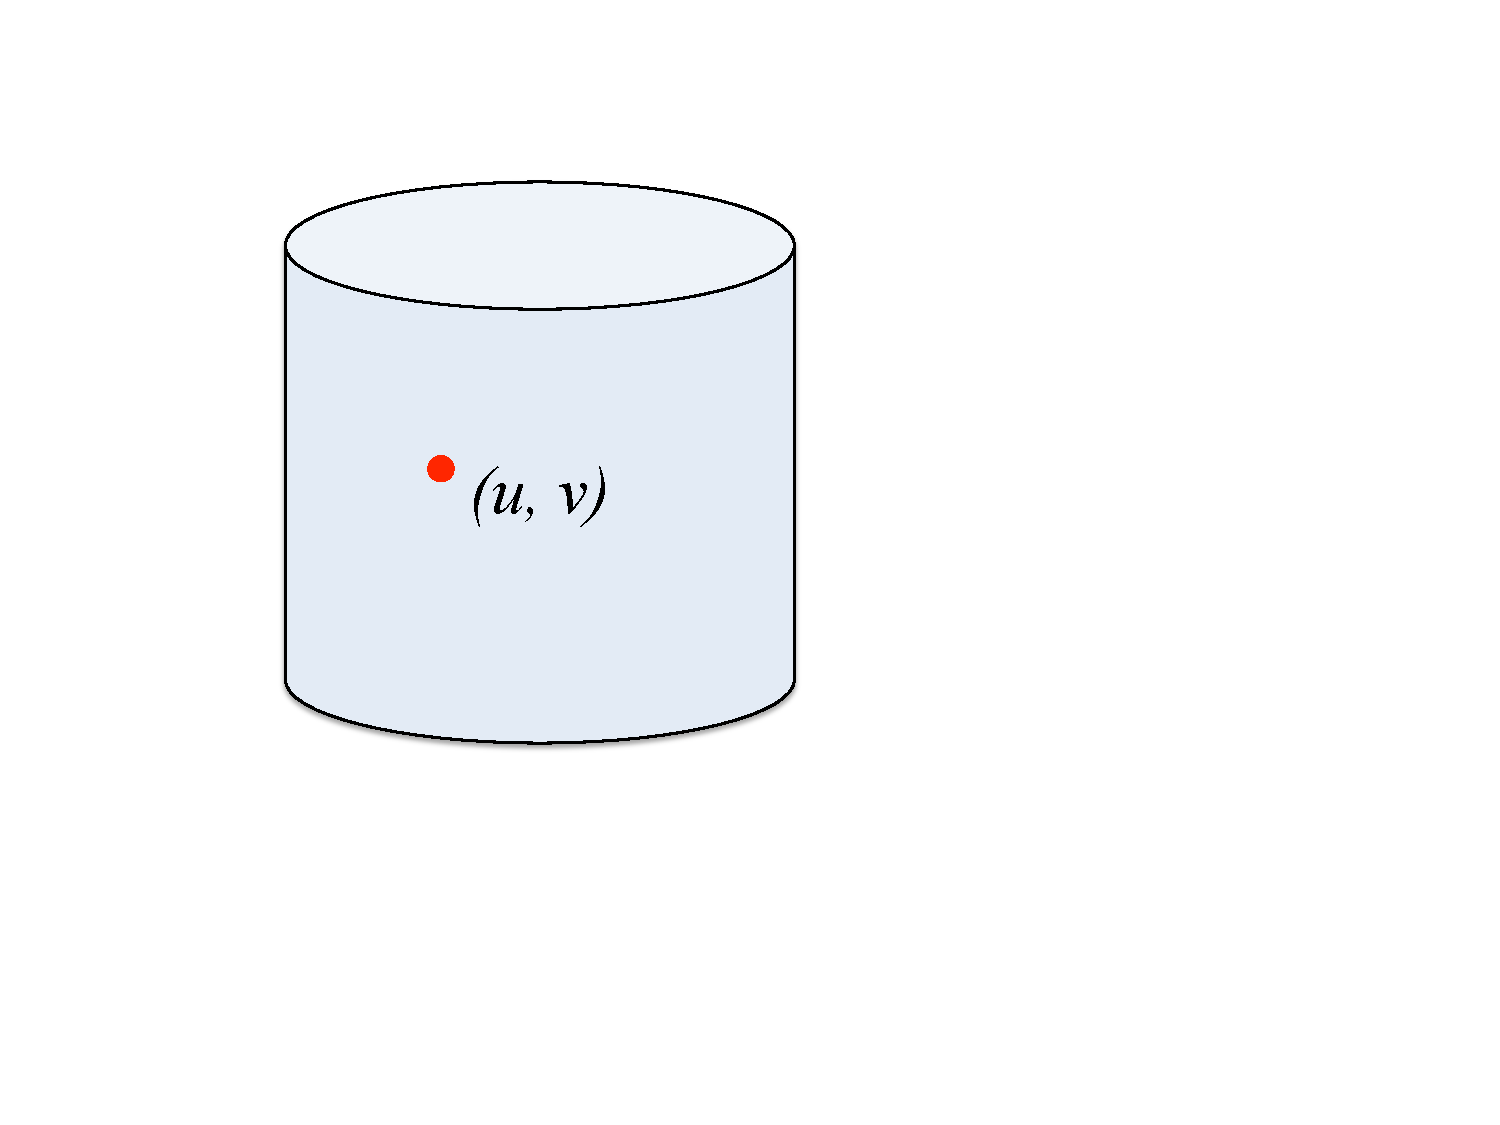
\includegraphics[width=\subwidth, clip=true, trim=130 125 300 30, page=1]{spider_cobweb}}
    %    \hfill
    %\subfigure[Offset feature]{%
        %\includegraphics[width=\subwidth, clip=true, trim=130 125 300 30, page=2]{spider_cobweb}
        %\label{subfig:cobweb}}
        %\hfill
    \subfigure[$\spiderfeat_1$]{%
        \includegraphics[width=\subwidth, clip=true, trim=130 105 300 30, page=4]{spider_cobweb}\label{subfig:c0}}
        \hfill
    \subfigure[$\spiderfeat_2$ (Top view)]{%
        \includegraphics[width=\subwidth, clip=true, trim=130 70 300 30, page=5]{spider_cobweb}\label{subfig:c1}}
        \hfill
    \subfigure[$\spiderfeat_3$ (Top view)]{%
        \includegraphics[width=\subwidth, clip=true, trim=130 70 300 30, page=6]{spider_cobweb}\label{subfig:c2}}
        \hfill
    \caption{
    %\todo{Add the tildes above the notation. I can fix this image on Friday when I am tired.}
    %(a) We compute a feature vector for a single point $\pixelidx = (u, v)$.
    %(b) The offset feature computes the difference in depth between $\pixelidx$ and the points that surround it.
    The spider features $\scalfeat_s(\pixelidx, \edgeimidx, \psi) = (s_1, s_2, s_3)$ provides three measures of the distance between $\pixelidx$ and the edge point $\edgeimidx$.
    (a) $s_1$ measures the distance between pixel locations $\pixelidx$ and $\edgeimidx$.
    (b) $s_2$ measures the distance between 3D points $\pointthreed$ and $\edgethreed$ along the surface of $\rgbdimage$.
    (c) $s_3$ gives an estimate of the depth of the object at the 3D location $\pointthreed$, using the surface normal $\mathbf{n}_\mathbf{s}$.
    }%
    \label{fig:features}
\end{figure}


%%%%%%%%%%%%%%%%%%%%%%%%%%%%%%%%%%%%%%%%%%
\subsection{The spider feature}
%\note{Name up for debate! Another candidate is `compass'}

\begin{wrapfigure}[7]{r}{0.45\columnwidth}
  \centering
  \vspace{-15pt}
    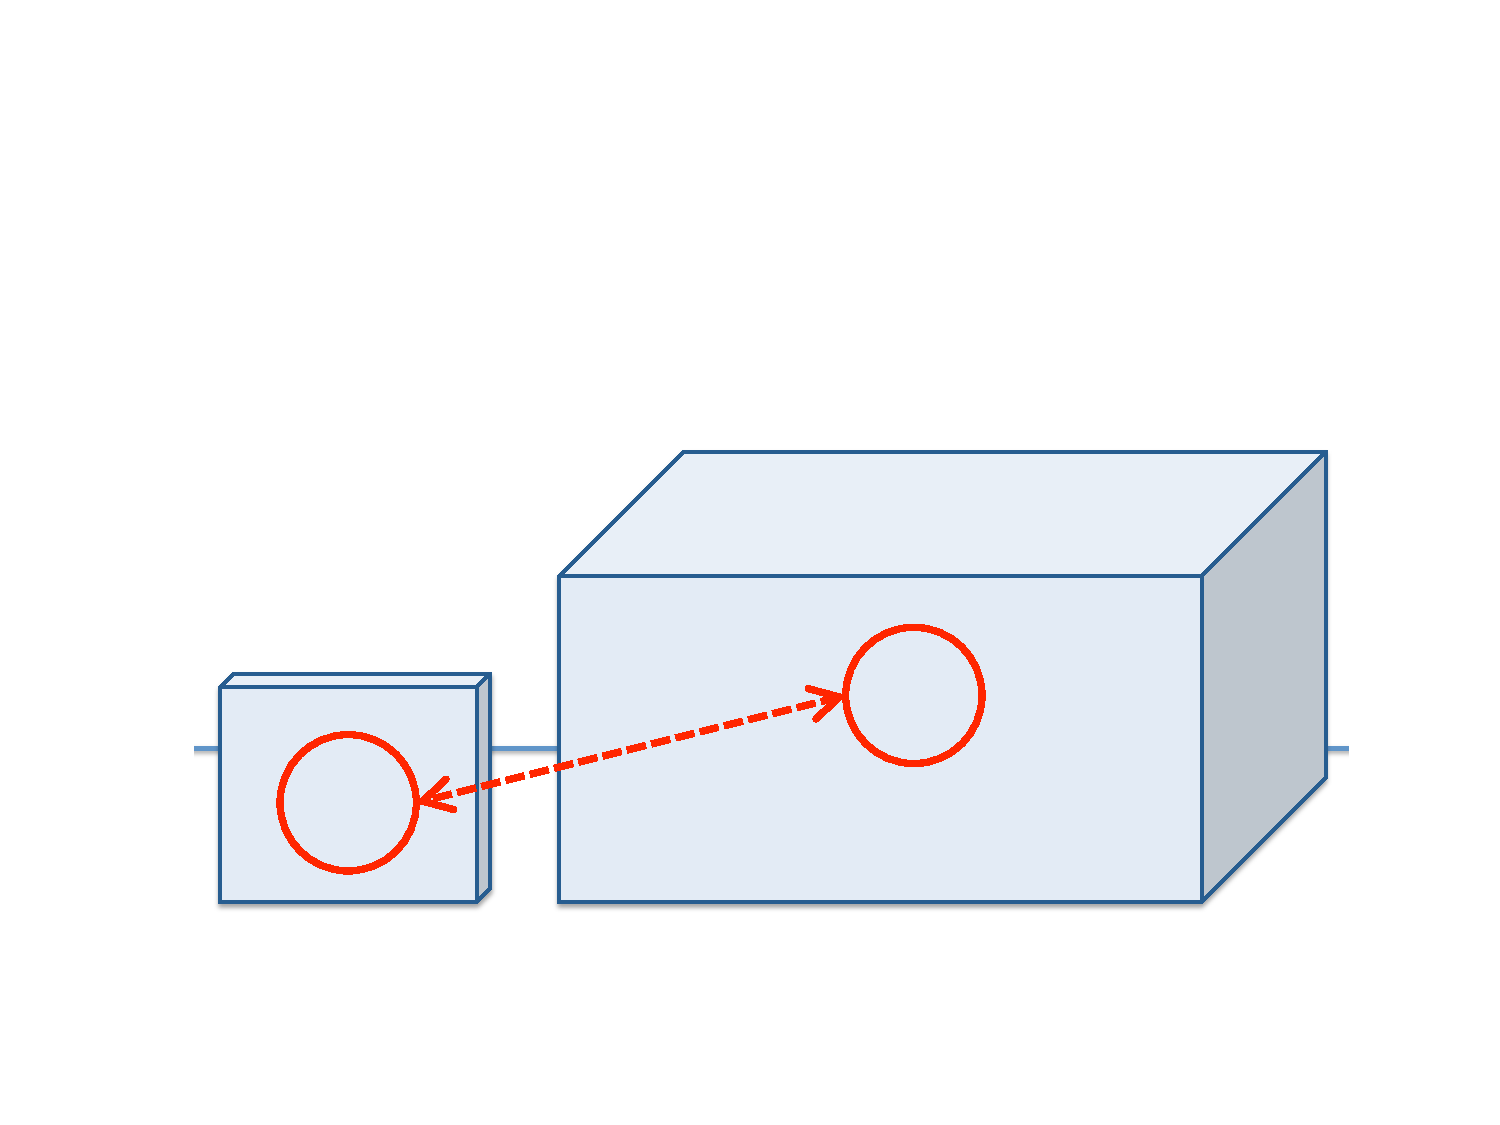
\includegraphics[width=0.45\columnwidth]{features_1}
    \vspace{-10pt}
  \caption{}%The offset feature}
    \label{fig:patch_problems}
\end{wrapfigure}
Local features, such as the offset feature, have proved discriminatory where the output labeling is on a per-pixel basis, such as labeling each pixel as a part of a human body \cite{shotton-cvpr-2011}.
However, when it comes to predicting the geometry of the scene we cannot observe, the local shape of the depth image around a point does not provide enough information.
An example of this can be seen in Figure \ref{fig:patch_problems}.
The two regions circled in the image have identical \emph{local} appearance, but the 3D geometry around each region is very different due to the different thicknesses of the two boxes.
We use this observation to motivate the `spider feature'.

  %vspace{-20pt}
% \begin{figure}[bt]
%   \centering
%   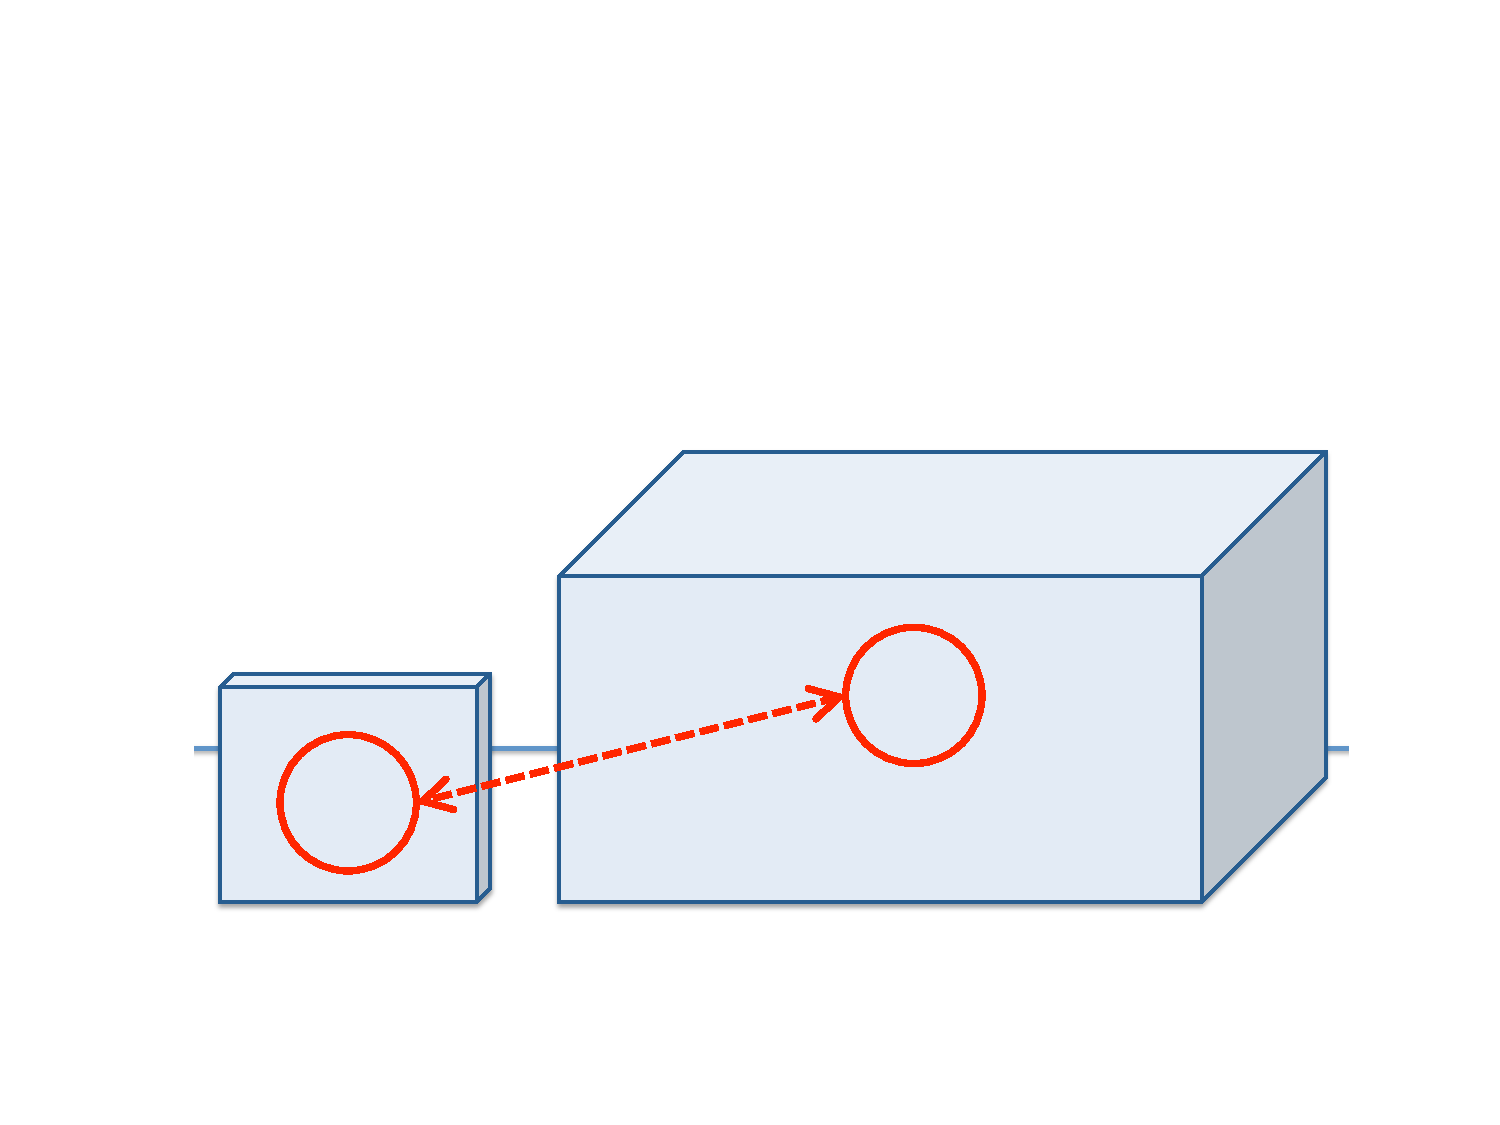
\includegraphics[width=0.9\columnwidth]{features_1}
%   \caption{Patch-type features do not give enough information to accurately predict depth. Here, regions on two different objects are marked. Each region has identical local appearance. However, the voxel geometry of the object at the two locations is very different due to the different thicknesses.
%   We use this observation to motivate the spider feature.}
%   \label{fig:patch_problems}
% \end{figure}
%\todo{Combine all the motivational images for the spider feature into one...}}


%Previous works have used the properties of a whole segmented region for classification of individual points \cite{golovinskiy-iccv-2009}.
%When it comes to predicting the 3D shape local to a point in a depth image, however, we care as much about the point's location in the region as we do about the overall region properties (Figure \ref{fig:spider_motivation}).

We desire a feature which captures the size and shape of the region in which $\pixelidx$ resides, along with the location of $\pixelidx$ in that region.
To achieve this we take inspiration from the features between a point and a binary edge map used by \cite{drost-3dimpvt-2012}.

\paragraph{Computing a binary edge map}
We first compute a binary edge map for the image, where each pixel takes the value 1 at a large change in depth or surface normal direction, and is 0 otherwise.
We first use the method of \cite{dollar-iccv-2013} to compute a real-valued edge map for the image. % (Figure \ref{subfig:structedge}).
Next we apply the Canny filtering algorithm \cite{canny-pami-1986} to convert this to a binary edge map. % (Figure \ref{subfig:binaryedge}).
We mitigate against poor quality depth data around discontinuities by dilating this edge map with a 3x3 disc-shaped structuring element.



\paragraph{Casting lines from $\pixelidx$}
From $\pixelidx$, we then cast a line across the edge map at angle $\psi$, where $\psi$ is a parameter of the feature computation.
We denote the point on the edge map where the line first hits a pixel with value 1 as $\edgeimidx$.
We additionally denote the 3D reprojections of the 2D pixel coordinates $\pixelidx$ and $\edgeimidx$ as $\pointthreed$ and $\edgethreed$ respectively.
%For each line cast we therefore have two points in 3D space: $\point$ and $\point_e$.

\paragraph{Extracting the spider feature}
The spider feature for a single point with a line cast in direction $\psi$ is $\scalfeat_s(\pixelidx, \edgeimidx, \psi) = (\spiderfeat_1, \spiderfeat_2, \spiderfeat_3)$.
Each element of this tuple is a distance between $\pixelidx$ and $\edgeimidx$, computed as follows:
\begin{itemize}

\item $\spiderfeat_1 = \rgbdimage(\pixelidx) \|\pixelidx - \edgeimidx\|_2 / f$. This is the distance between $\pixelidx$ and $\edgeimidx$ in pixel units $\|\pixelidx - \edgeimidx\|_2$ scaled by $\rgbdimage(\pixelidx) / f$ to convert to a real-world distance (Figure \ref{subfig:c0}).

\item $\spiderfeat_2 = \sum_{i=2}^{|\gline|} \| \gline(i) - \gline(i-1)) \|_2 $, where $\gline$ is an ordered list of the 3D locations of the points on the line between $\pixelidx$ and $\edgeimidx$.
$\spiderfeat_2$ approximates the arc length between $\pixelidx$ and $\edgeimidx$ along the surface of $\rgbdimage$  (Figure \ref{subfig:c1}).

\item $\spiderfeat_3 = (\pointthreed - \edgethreed) \cdot \normal_\pixelidx$.
This is the Euclidean distance between 3D points $\pointthreed$ and $\edgethreed$ along the direction of the normal $\normal_\pixelidx$ at $\pixelidx$  (Figure \ref{subfig:c2}).

\end{itemize}

We compute $\scalfeat_s(\pixelidx, \edgeimidx, \psi)$ for  $\psi \in \{0\degree, 45\degree, \ldots, 315\degree\}$, and concatenate the results into a  24-dimensional vector $\feat_{\text{spi}}$.
The concatenation of $\feat_\text{off}$ and $\feat_\text{spi}$ forms the final 56D feature vector $\feat(\pixelidx)$ for point $\pixelidx$.

\paragraph{Implementation}
The spider feature is efficient to compute; we can compute the 24D spider feature for every point in a $640\times480$ image in less than 0.01s using our C++ implementation.
%We would expect a significant speedup were this to be implemented on a GPU.


% \paragraph{Occluded spider features}
% \todo{Remove or improve and do experiments}

% We explicitly handle occlusion in the spider features. Where the spider feature first hits an occluded edge rather than an occluding edge, the true size of the object in that dimension is unknown (see figure \ref{fig:features:occluded_spider}).
% However, we do have a \textit{minimum} size in that direction.

% We reason that discontinuities in depth images can be assigned a direction: one side of each edge is the occluder, the other is the occludee.
% We can compute the gradient of the depth edges using PCA on the edge pixels in image space.
% We ensure that the final gradient at each edge pixel points in the direction of the occluded side.

% We can then use the occlusion information in our feature computations.
% See for example figure \ref{fig:occluded_region}.


% \begin{figure}
%     \centering
%     \subfigure[]{%
%         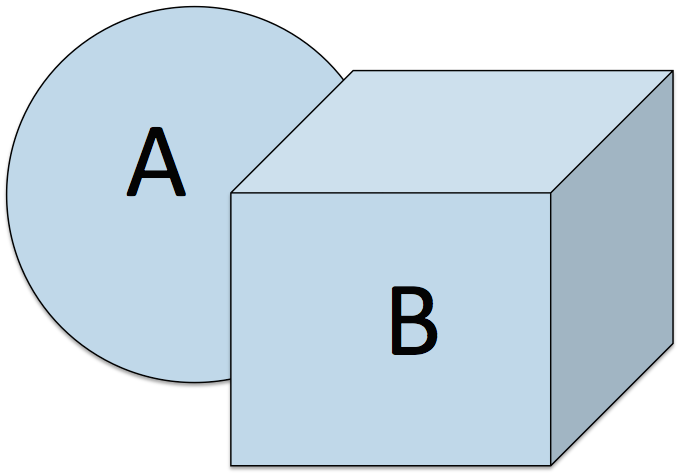
\includegraphics[width=0.45\columnwidth]{occlusion_a}}
%         \hfill
%     \subfigure[]{%
%         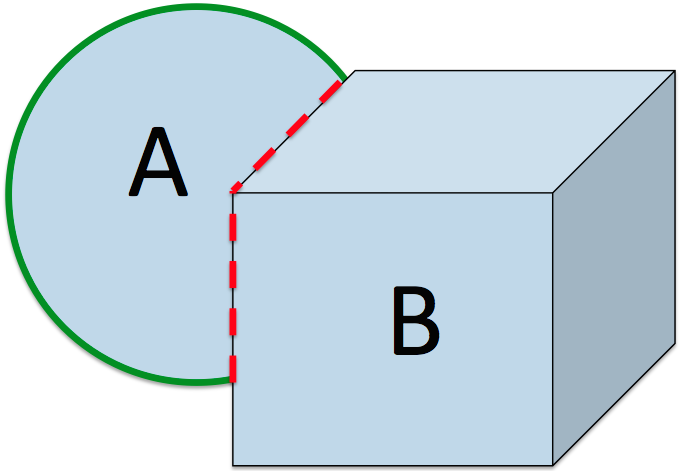
\includegraphics[width=0.45\columnwidth]{occlusion_b}} \\
%     \caption{Where edges occur as a result of occlusion boundaries, the direction of the edge is important. The edge bounding region A can be divided into an \emph{occluding} portion (solid green) and an \emph{occluded} portion (dashed red).
%     We can make a reasonable assumption that region A may extend behind object B past the occluded edge.
%     However, region A cannot continue sideways beyond its occluding edge.}
%     \label{fig:occluded_region}
% \end{figure}

% \begin{figure}
%     \centering%
%     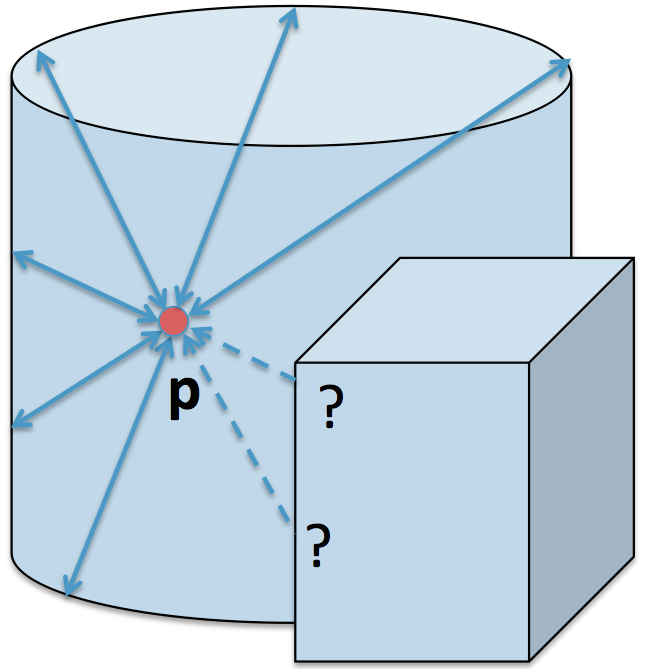
\includegraphics[width=0.7\columnwidth]{occlusion_spider.png}%
%     \figcaption{The spider feature extends lines from $\point$ to the first occluding edge found along the path. Internal edges (e.g. those found in RGB space) are ignored. Where the line first hits an occluded edge, the true extent is unknown --- this case is denoted as \texttt{?} in this figure.}%
%     \label{fig:occluded_spider}%
% \end{figure}


% %%%%%%%%%%%%%%%%%%%%%%%%%%%%%%%%%%%%%%%%%%%%%%%%%%%%%%%%%%%%%%%%%%%%%%%%%%%%%%%%
\section{Learning a mapping from features to voxlets}
\label{sec:forest_train}
% %%%%%%%%%%%%%%%%%%%%%%%%%%%%%%%%%%%%%%%%%%%%%%%%%%%%%%%%%%%%%%%%%%%%%%%%%%%%%%%%
In this paper we pose unobserved geometry estimation given partial observed information as a supervised learning problem.
More specifically, our goal is to learn a function $f: \mathcal{X}\to \mathcal{Y}$, which maps each observed feature vector $\mathbf{x} \in \mathcal{X}$ to the label space $\mathbf{v} \in \mathcal{Y}$ representing the corresponding 3D geometry in the region $\mathcal{R}$ around $\mathbf{x}$.
Unlike standard classification where the goal is to predict a category label for each $\mathbf{x}$, our label space is a multi-dimensional structured vector $\mathbf{v} \in \mathbb{R}^{w\times{}d\times{}h}$ which encodes the TDSF values in a local region.
Inspired by the recent work of Doll{\'a}r and Zitnick~\cite{dollar-iccv-2013} we use a structured Random Forest to learn the function $f$.

\paragraph{Training}
To train the forest we pass a bagged subset of the training set $\left\{(\mathbf{x}_1, \mathbf{v}_1), ..., (\mathbf{x}_n, \mathbf{v}_n)\right\}$ to each node in the tree starting at the root.
Each node is then tasked with splitting the examples so that the ones sent to its children are as similar as possible in label space.
Instead of minimizing the structured loss directly, Doll{\'a}r and Zitnick~\cite{dollar-iccv-2013} approximate this loss at each node using a classification loss.
To convert the structured problem into a classification one we sample a different random subset of the dimensions of each $\mathbf{v}_i$ at the node, reduce their dimensionality to $N$ dimensions, and then cluster them into a discrete number of classes $K$ (here we set $N=20$ and $K=2$).
Then a standard classification loss can be used on this new discretization to evaluate the quality of different candidate splits for each $\mathbf{x}_i$.
In practice, this dimensionality reduction and clustering can be efficiently performed using randomized PCA~\cite{halko-siam-2011}.
To cluster, a training example is assigned to one of the two possible clusters $K$ based on the sign of the values in its first principal component.

This process is repeated until we cannot split the data any further.
Finally, each leaf node stores the medoid of all the examples that have arrived there, which we refer to as a voxlet, see Figure \ref{fig:voxlets}.

%$k$ = $min_k\sum_j(\mathbf{v}_{kj} - \bar{\mathbf{v}}_j)^2$

\paragraph{Testing}
Evaluating each tree at test time is extremely efficient.
For each location in the input depth image we simply traverse the tree until we reach a leaf node and return the voxlet stored at that location, see Figure \ref{subfig:forest_overview}.

\paragraph{Implementation}
Given the large dimensionality of $\mathcal{Y}$ we perform an initial dimensionality reduction to a 50 dimensional space using PCA.
Due to the large amount of redundancy in each $\mathbf{v}$ we found this to have little impact on the quality of our results, and yet it provides a large improvement to computational tractability.
We use an ensemble of 50 trees, which are grown to a maximum depth of 15 or until there is a minimum of 2 examples at a node.
We use simple axis aligned feature splits at each node.

\newcommand{\voxletsubwidth}{0.41\columnwidth}
\begin{figure}
     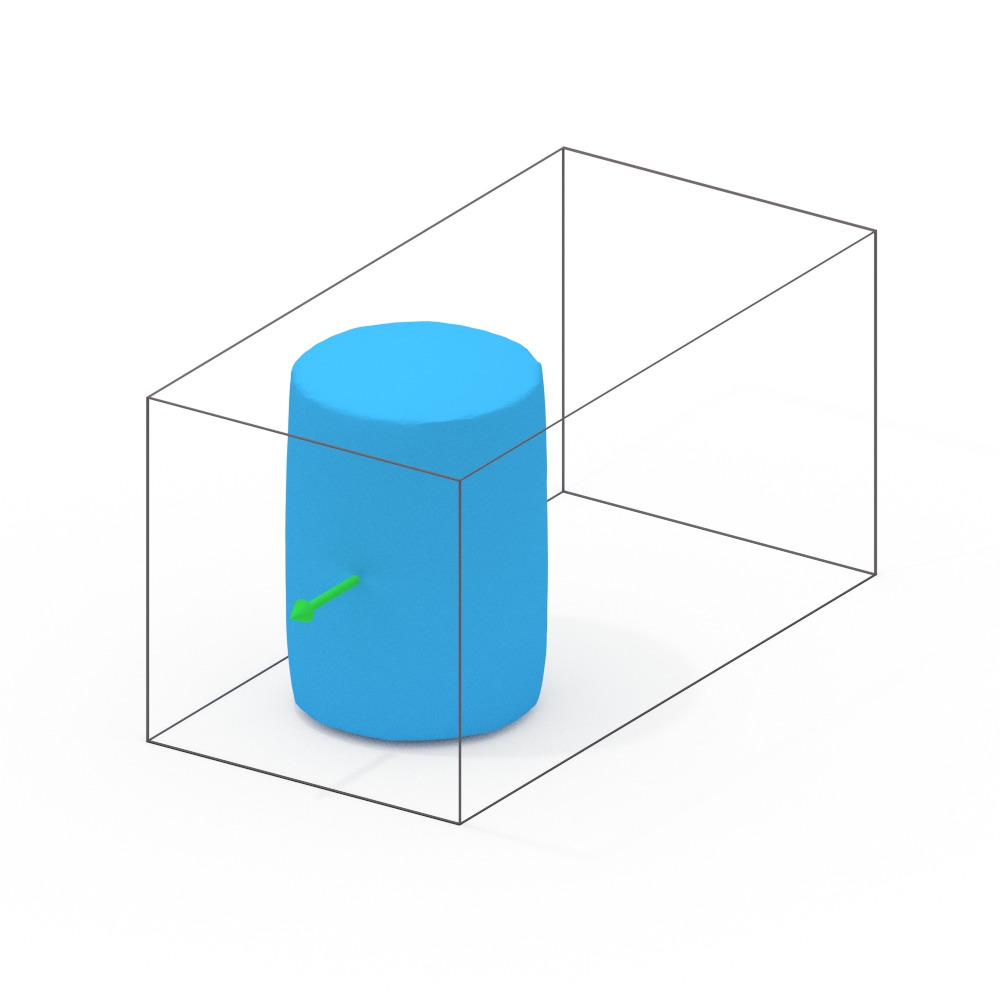
\includegraphics[width=0.32\columnwidth, clip=true, trim=130 150 120 150]{data/all_voxlets_renders_white/1_marching_cubes.jpg}
     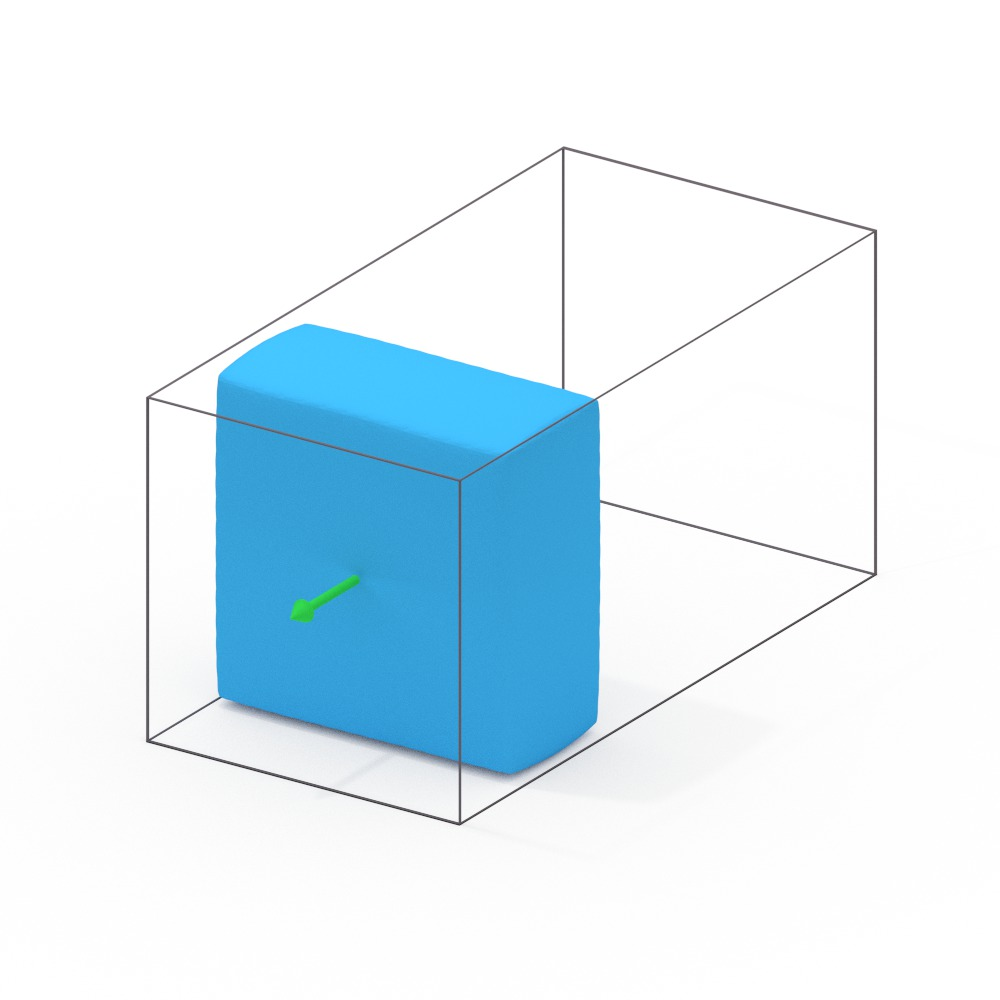
\includegraphics[width=0.32\columnwidth, clip=true, trim=130 150 120 150]{data/all_voxlets_renders_white/5_marching_cubes.jpg}
     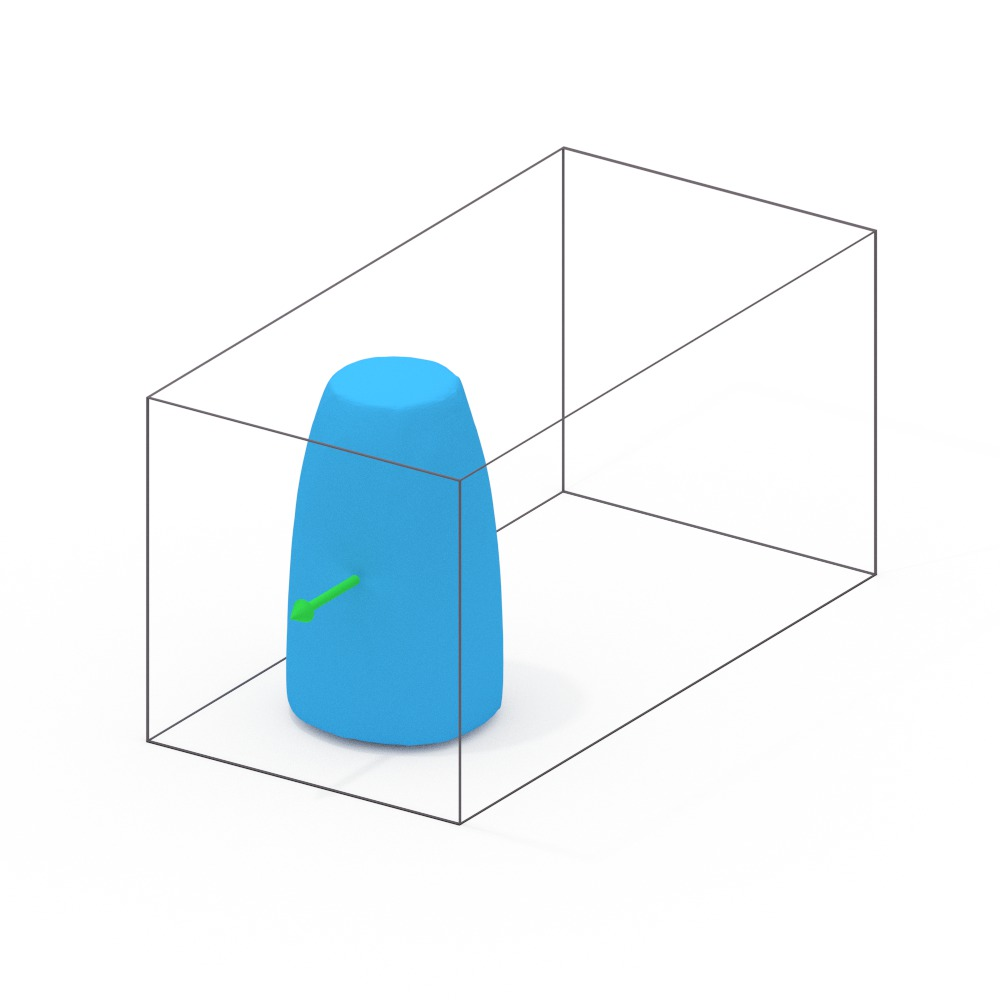
\includegraphics[width=0.32\columnwidth, clip=true, trim=130 150 120 150]{data/all_voxlets_renders_white/10_marching_cubes.jpg} \\
     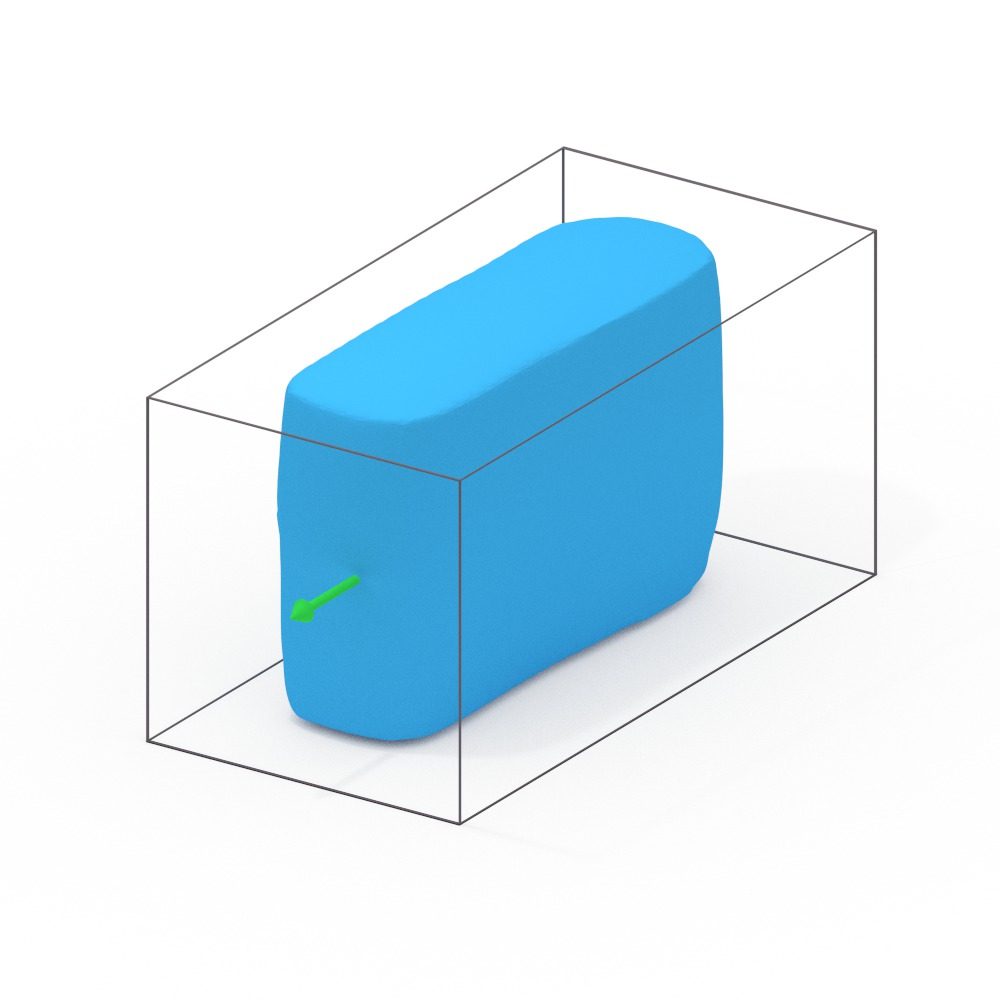
\includegraphics[width=0.32\columnwidth, clip=true, trim=130 150 120 150]{data/all_voxlets_renders_white/95_marching_cubes.jpg}
     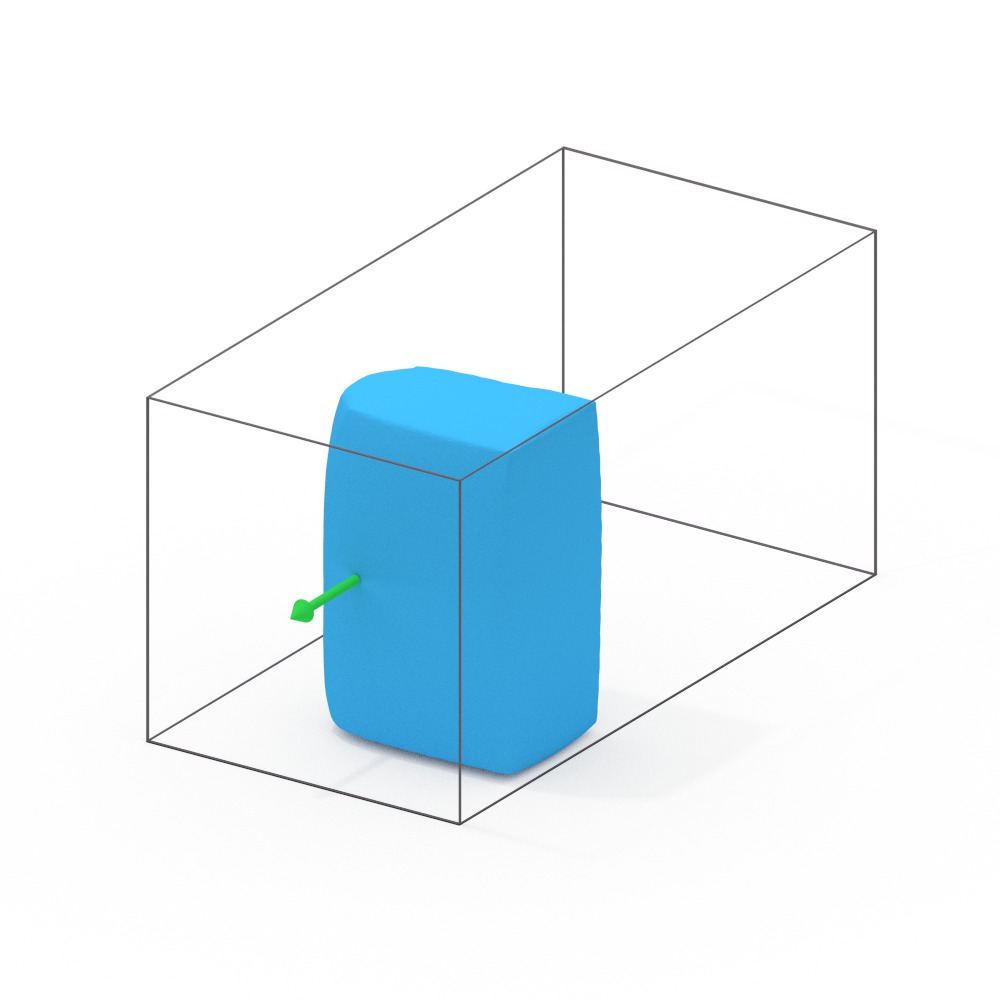
\includegraphics[width=0.32\columnwidth, clip=true, trim=130 150 120 150]{data/all_voxlets_renders_white/38_marching_cubes.jpg}
     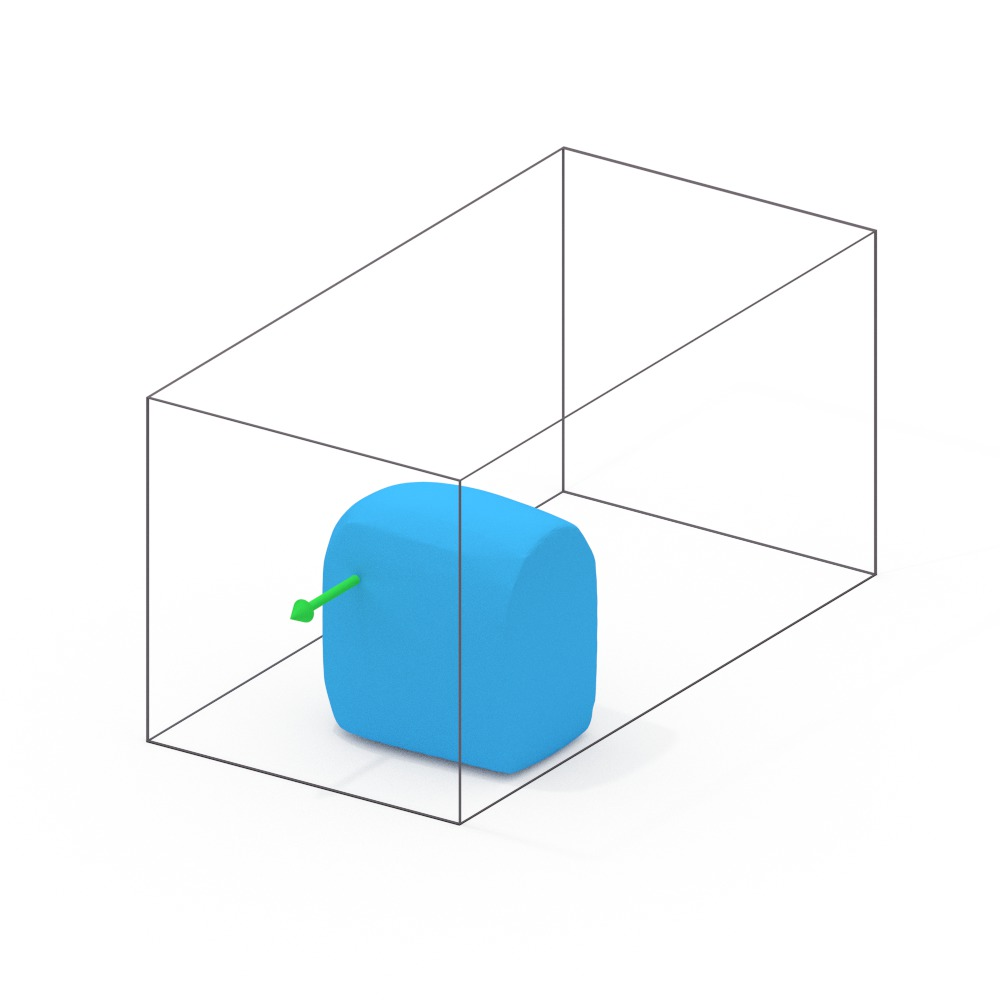
\includegraphics[width=0.32\columnwidth, clip=true, trim=130 150 120 150]{data/all_voxlets_renders_white/44_marching_cubes.jpg}
     \caption{Representative voxlets from the dataset. Here we show cluster centroids after running K-Means on a collection of 20,000 voxlets, with K=200.
     The green arrow represents the vector which is aligned with $\mathbf{n}_\mathbf{s}$ (see Figure \ref{subfig:alignment}).
     Each voxlet can be seen to capture a section of the geometry of an object.}
     \label{fig:voxlets}
\end{figure}



%\note{Our training set is extracted from ...
%We set size of $\mathcal{R}$ to $15, 15, 30$ ...}

\pagedepth\maxdimen
\subsection{The voxlet dimensions}
\begin{wrapfigure}[10]{r}{0.35\columnwidth}
  \vspace{-30pt}
  \centering
    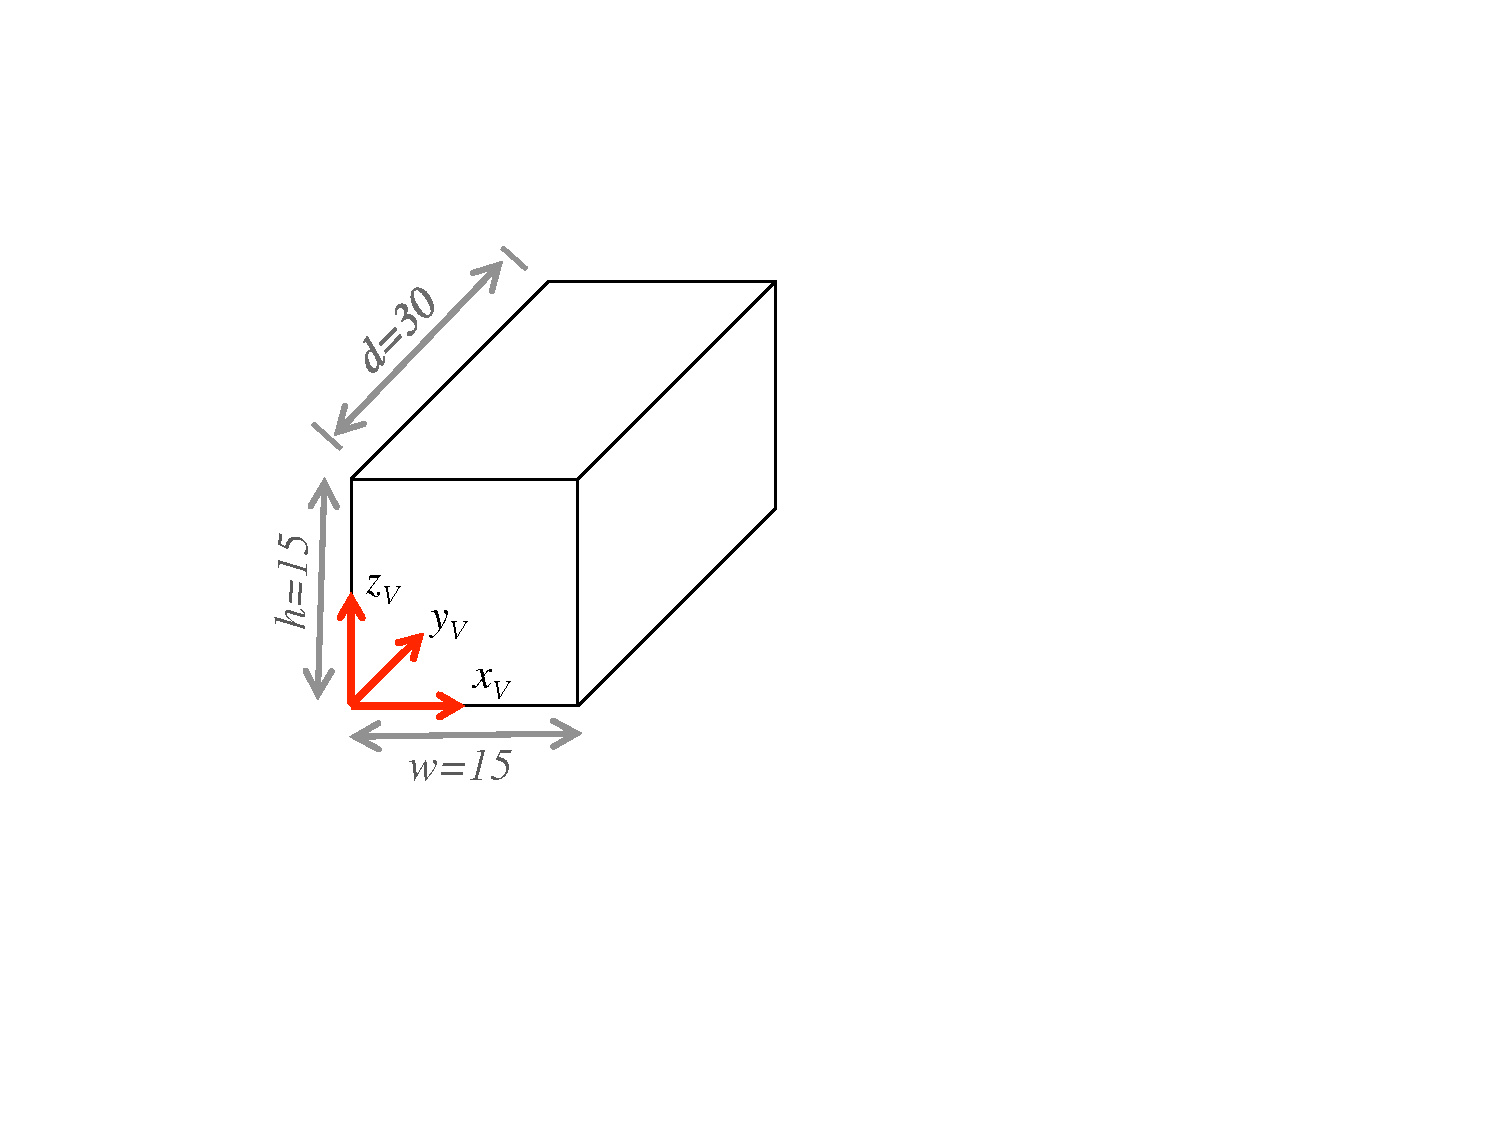
\includegraphics[width=0.35\columnwidth, clip=true, trim=120 140 340 80]{single_voxlet}
    \vspace{-15pt}
  \caption{}%The offset feature}
    \label{fig:voxlet_dims}
\end{wrapfigure}
The fixed-size regions $\mathcal{R}$ in the voxel grid are set in our experiments to have dimensions of $15 \times 30 \times 15$ voxels.
We make the voxlets longer in the y-direction as it is this direction that is approximately parallel to the normal at $\pixelidx_p$.
This allows the voxlet to make a larger prediction \emph{backwards} into the scene than \emph{sideways} into a region which typically already has observed data.
We set each voxlet to have real-world dimensions $0.1m \times 0.2m \times 0.1m$, meaning each voxel inside a voxlet has edge lengths of $(0.1 / 15)$m.
We define a local coordinate system for the voxlet, as shown in red in Figure \ref{fig:voxlet_dims}.
The position in the voxlet which we align with the 3D point $\pixelidx_p$, as shown in Figure \ref{subfig:alignment}, is the point $x_v = y_v = z_v = 0.05$m.



%%%%%%%%%%%%%%%%%%%%%%%%%%%%%%%%%%%%%%%%%%%%%%%%%%%%%%%%%%%%%%%%%%%%%%%%%%%%%%%%
\subsection{Aggregating predictions}
\label{sec:combining}
%%%%%%%%%%%%%%%%%%%%%%%%%%%%%%%%%%%%%%%%%%%%%%%%%%%%%%%%%%%%%%%%%%%%%%%%%%%%%%%%

For each voxel in the output grid $\voxelgrid$, we accumulate the predictions of the multiple overlapping TSDF predictions at that location.
A number of different strategies could be employed to recover our final values, \eg filtering techniques, loopy belief propagation \etc.
In our work we simply take the mean of all the predictions at that voxel.
We note that the truncation of the signed distance function helps to make this style of accumulation robust.
A single incorrect estimation at a voxel can only be wrong by a maximum amount of $2d_{\max}$, where $d_{\max}$ is the level at which the distance function is truncated.

Some voxels in $\voxelgrid$ do not have any predictions made for them at all.
We assign to these voxels the value $d_{\max}$.

The final TSDF estimation can be converted to a mesh by finding the level-set of zero, for example using marching cubes \cite{lorensen-siggraph-2013}.


%%%%%%%%%%%%%%%%%%%%%%%%%%%%%%%%%%%%%%%%%%%%%%%%%%%%%%%%%%%%%%%%%%%%%%%%%%%%%%%%
\section{Experiments}
%%%%%%%%%%%%%%%%%%%%%%%%%%%%%%%%%%%%%%%%%%%%%%%%%%%%%%%%%%%%%%%%%%%%%%%%%%%%%%%%

We evaluate our algorithm from the perspective of its ability to reconstruct objects in isolation, and then further its ability to reconstruct more cluttered scenes.
All of the experiments are performed on data captured from the Microsoft Kinect.



%%%%%%%%%%%%%%%%%%%%%%%%%%%%%%%%%%%%%%%%%%%%%%%%%%%%%%%%%%%%%%%%%%%%%%%%%%%%%%%%
\subsection{Experimental procedure}

In our experiments we first smooth the noisy depth data using cross-bilateral filtering, using the implementation provided by \cite{silberman-eccv-2012}.
We then detect the largest approximately horizontal plane in the image, and use this to estimate the `up' direction of the scene.
We make an estimate of geometry using the 3D points which lie above this detected planar surface.

%A parameter of our  is how many pixels to evaluate.
We can choose at test time how many pixels to run through the forest to make a prediction of voxel occupancy.
In our experiments we use 200 pixels.
The forest predictions for these pixels are then aggregated as described in Section \ref{sec:combining}.


%%%%%%%%%%%%%%%%%%%%%%%%%%%%%%%%%%%%%%%%%%%%%%%%%%%%%%%%%%%%%%%%%%%%%%%%%%%%%%%%
%\subsection{Datasets used}


\subsection{Datasets}
We introduce two datasets to evaluate our algorithm, both of which will be placed in the public domain.

% \paragraph{Synthetic dataset D1}
Our \textbf{synthetic dataset (D1)} is a is a large dataset of 500 scenes, each featuring a random arrangement of CAD primitives.
These random but physically plausible arrangements were formed by dropping objects onto a plane using a physics simulator. Each scene is then rendered from 42 viewpoints in a hemisphere.
This large dataset allows us to easily quantify the effects of various parts of our algorithm, and to demonstrate the various stages of the algorithm.

%\paragraph{Desks dataset D2}
Existing RGBD datasets of natural scenes typically focus on the per-frame labelling task \cite{nyu, sun3d}, object detection \cite{rgbd scenes dataset} or camera pose estimation \cite{stanford?}.
There are no datasets to our knowledge which have the aim of capturing the full geometry of a scene.
We therefore introduce a \textbf{desktop dataset (D2)}, capturing the full geometry of [75] desktops in an office.
The desks were not manipulated before data capture, meaning they include the true intricacies of the real world.
This dataset has wide applications in geometry recovery, mesh segmentation and reconstruction.
We include the raw color and depth frames, together with the reconstructed mesh and voxelised volume for the data.


%Example images from this dataset are shown in Figure \ref{fig:osm}.


\begin{table}
  \centering
  \begin{tabular}{|p{4.8cm}|c|c|}
  %\toprule
  \hline
  \textbf{Method}  &   \textbf{Precision} & \textbf{Recall} \\
  \hline
  %\midrule
  Bounding box & 0.550 & 0.683  \\
  Zheng \ea \cite{zheng-cvpr-2013}  & 0.570 & 0.466 \\
  K-means forest & 0.922 & 0.944 \\
  Structured forest (offset only) & 0.921 & 0.948 \\
  Structured forest (spider only) &  0.855 & 0.949 \\
  Structured forest (offset + spider) & 0.926 & 0.948 \\
  \hline
  %\bottomrule
  \end{tabular}
  \vspace{5pt}
  \caption{A comparison of the accuracy of geometry estimation algorithms on the Bigbird dataset. Details of the algorithms used are given in Section \ref{sec:algorithms}.}
    \label{tab:quant_results}
\end{table}


%%%%%%%%%%%%%%%%%%%%%%%%%%%%%%%%%%%%%%%%%%%%
\subsection{Quantitative evaluation}

\paragraph{Evaluation criteria}
The aim of our algorithm is to accurately classify free space around objects and in scenes.
Therefore, we report the per-voxel precision and recall over all the test data.
For our algorithms, we use the sign of the accumulated TSDF to form our final binary prediction of occupancy.

%To find our test volume, we find the minimum volume axis-aligned bounding box for the ground truth voxel data before padding this voxel grid with 10cm of padding in each axis direction.


\paragraph{Baselines and algorithm variants}
\label{sec:algorithms}
We compare to two main baseline algorithms: a naive bounding box approach and the method of Zheng \ea \cite{zheng-cvpr-2013}.
The details of these baseline implementations, and of the details of variants of our method, are:

\noindent \textbf{(a) Bounding box} We fit a minimum-area bounding box to the 3D points belonging to the object, as defined by the ground truth object segmentation mask provided by \cite{singh-icra-2014}.
We are careful to remove `flying pixels', as they can have a large adverse effect on bounding box predictions.
Finally, the prediction of voxel occupancy is simply all voxels inside the bounding box are predicted to be occupied, while those outside are predicted to be empty.

\noindent \textbf{(b) Zheng \ea} \cite{zheng-cvpr-2013}
We implemented the algorithm of Zheng \ea \cite{zheng-cvpr-2013} for reconstructing voxel occupancy as described in Section 2 of their paper.
We find the Manhattan axes of the scene from the minimum area bounding box aligned with the ground truth voxel grid.
We then perform their axis-aligned voxel search for each unobserved voxel, marking voxels as `filled' where more than two Manhattan directions hit a voxel directly observed by the camera.

%We consider this to be a best-case implementation of object-wise Manhattan-world estimation.

%We do not implement their method for physical reasoning of objects  as we are making predictions for single objects in isolation.

\noindent \textbf{(c) K-means forest} We train a standard classification Random Forest, the leaf nodes of which vote for items in a dictionary of 200 voxlets formed by running K-means on the training set of voxlets. The transformation into the scene and the aggregation steps are equivalent to our core algorithm.

\noindent \textbf{(d) Structured (offset only)} Our full structured forest, but only using the offset features

\noindent \textbf{(e) Structured (spider only)} Our full structured forest, but only using the spider features

\noindent \textbf{(f) Structured (offset + spider)}  Our full structured forest using both offset and spider features.

\vspace{10pt}

The results from our quantitative analysis on the Bigbird turntable dataset are shown in Table \ref{tab:quant_results}.
We present some views of individual results in Figure \ref{fig:turntable_qual}.
We notice that the naive bounding box prediction suffers from a poor rate of recall.
This is expected, as typically the bounding box predictions under-predict the volume due to a lack of observed pixels to complete the shape of the object (\ref{fig:turntable_qual}).
Our results successfully capture the overall geometry of each of the objects.
The main, general point of failure is a smoothing effect which affects the edges of the objects.

While our full forest outperforms the other methods, we notice only a small change in the variants of our approach using different features.
The lower precision and higher recall for the spider feature suggests that it is over-predicting the size of objects, although the performance is maximized when it is coupled with the offset feature.
The K-means Forest does almost as well as our full structured forest.
However, as it has discretized the label space before training we would not expect it to generalize well to larger and more diverse training data.


\newcommand{\turnheight}{0.26\columnwidth}
\begin{figure*}
    \begin{tabular}{cccccc}
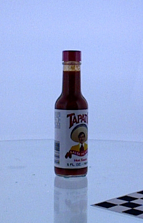
\includegraphics[height=\turnheight, clip=true, trim=30 30 30 30]{data/rgb_ims/tapatio_hot_sauce} &
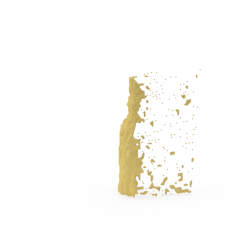
\includegraphics[height=\turnheight, clip=true, trim=60 30 30 60]{data/renders_turn_table/tapatio_hot_sauce_NP1_312.mat_visible_pixels_view_90} &
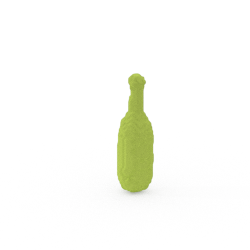
\includegraphics[height=\turnheight, clip=true, trim=60 30 30 60]{data/renders_turn_table/tapatio_hot_sauce_NP1_312.mat_gt_view_90} &
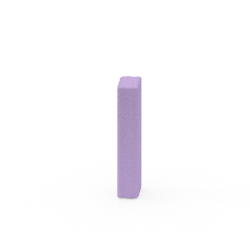
\includegraphics[height=\turnheight, clip=true, trim=60 30 30 60]{data/renders_turn_table/tapatio_hot_sauce_NP1_312.mat_bb_view_90} &
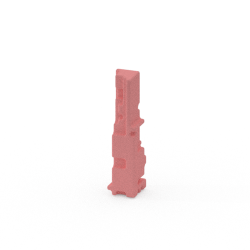
\includegraphics[height=\turnheight, clip=true, trim=60 30 30 60]{data/renders_turn_table/tapatio_hot_sauce_NP1_312.mat_zheng_view_90} &
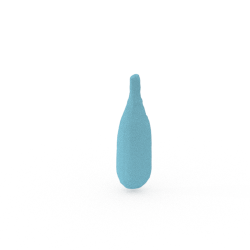
\includegraphics[height=\turnheight, clip=true, trim=60 30 30 60]{data/renders_turn_table/tapatio_hot_sauce_NP1_312.mat_oma_view_90} \\
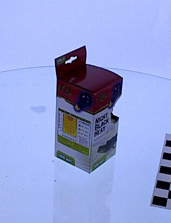
\includegraphics[height=\turnheight, clip=true, trim=30 30 30 30]{data/rgb_ims/zilla_night_black_heat} &
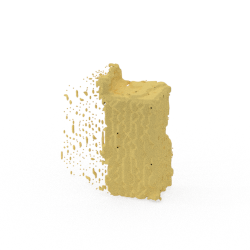
\includegraphics[height=\turnheight, clip=true, trim=60 30 30 60]{data/renders_turn_table/zilla_night_black_heat_NP2_312.mat_visible_pixels_view_180} &
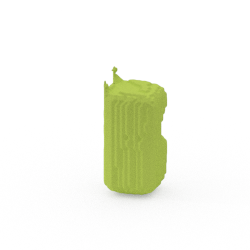
\includegraphics[height=\turnheight, clip=true, trim=60 30 30 60]{data/renders_turn_table/zilla_night_black_heat_NP2_312.mat_gt_view_180} &
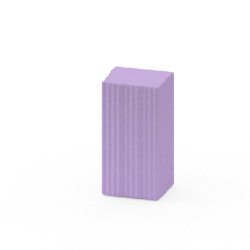
\includegraphics[height=\turnheight, clip=true, trim=60 30 30 60]{data/renders_turn_table/zilla_night_black_heat_NP2_312.mat_bb_view_180} &
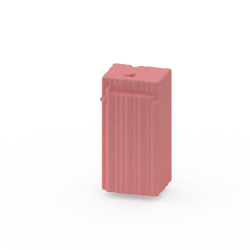
\includegraphics[height=\turnheight, clip=true, trim=60 30 30 60]{data/renders_turn_table/zilla_night_black_heat_NP2_312.mat_zheng_view_180} &
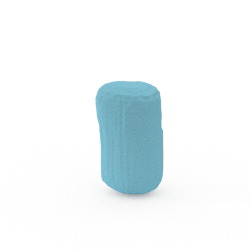
\includegraphics[height=\turnheight, clip=true, trim=60 30 30 60]{data/renders_turn_table/zilla_night_black_heat_NP2_312.mat_oma_view_180} \\
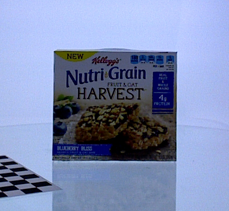
\includegraphics[height=\turnheight, clip=true, trim=30 30 30 30]{data/rgb_ims/nutrigrain_harvest_blueberry_bliss} &
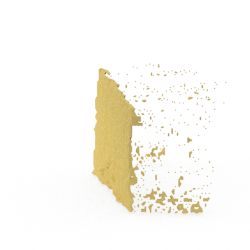
\includegraphics[height=\turnheight, clip=true, trim=60 30 30 60]{data/renders_turn_table/nutrigrain_harvest_blueberry_bliss_NP1_0.mat_visible_pixels_view_0} &
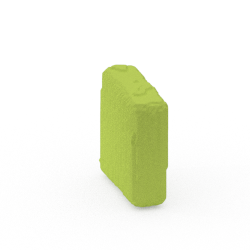
\includegraphics[height=\turnheight, clip=true, trim=60 30 30 60]{data/renders_turn_table/nutrigrain_harvest_blueberry_bliss_NP1_0.mat_gt_view_0} &
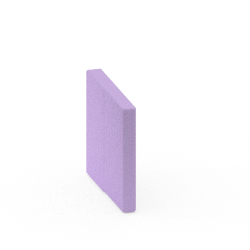
\includegraphics[height=\turnheight, clip=true, trim=60 30 30 60]{data/renders_turn_table/nutrigrain_harvest_blueberry_bliss_NP1_0.mat_bb_view_0} &
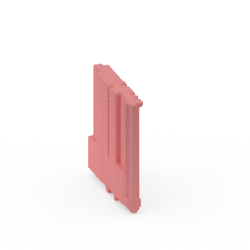
\includegraphics[height=\turnheight, clip=true, trim=60 30 30 60]{data/renders_turn_table/nutrigrain_harvest_blueberry_bliss_NP1_0.mat_zheng_view_0} &
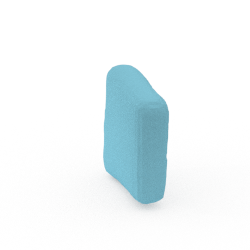
\includegraphics[height=\turnheight, clip=true, trim=60 30 30 60]{data/renders_turn_table/nutrigrain_harvest_blueberry_bliss_NP1_0.mat_oma_view_0} \\
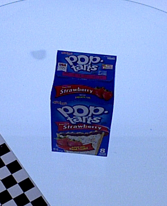
\includegraphics[height=\turnheight, clip=true, trim=30 30 30 30]{data/rgb_ims/pop_tarts_strawberry} &
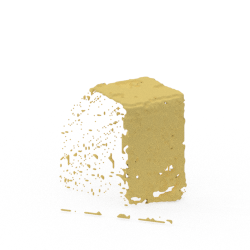
\includegraphics[height=\turnheight, clip=true, trim=60 30 30 60]{data/renders_turn_table/pop_tarts_strawberry_NP3_0.mat_visible_pixels_view_90} &
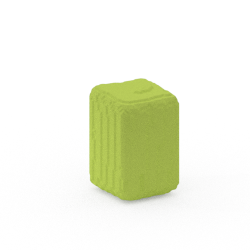
\includegraphics[height=\turnheight, clip=true, trim=60 30 30 60]{data/renders_turn_table/pop_tarts_strawberry_NP3_0.mat_gt_view_90} &
\includegraphics[height=\turnheight, clip=true, trim=60 30 30 60]{data/renders_turn_table/pop_tarts_strawberry_NP3_0.mat_bb_view_90} &
\includegraphics[height=\turnheight, clip=true, trim=60 30 30 60]{data/renders_turn_table/pop_tarts_strawberry_NP3_0.mat_zheng_view_90} &
\includegraphics[height=\turnheight, clip=true, trim=60 30 30 60]{data/renders_turn_table/pop_tarts_strawberry_NP3_0.mat_oma_view_90} \\
     Input view & Input depth pixels & Ground truth mesh & Bounding box &  Zheng \ea & Our result \\
    \end{tabular}
    \vspace{5pt}
     \caption{Results from the Bigbird turntable dataset.
     Each row shows a different object, while each column shows the result of a different algorithm.
      The first column shows the RGB image of the input view, while the second column shows the reprojected input depth pixels from a side view.
     The following columns, all shown from the same viewpoint as the input depth pixels view, demonstrate the different baselines and algorithm variants.
      More views and objects can be seen in the supplementary material.
     \label{fig:turntable_qual}
     }
\end{figure*}
     %Our algorithm is able to predict shape beyond the extents of the visible depth pixels, and can also recover the shape of non-prismoidal objects, such as in the first row.
% (a) Input view &
     %For visualization purposes we have converted the voxel grids to a mesh using marching cubes.
     %The details of the algorithms are given in Section \ref{sec:algorithms}, and


% \begin{figure*}
%     \begin{tabular}{cccc}



%      \includegraphics[width=0.32\columnwidth, clip=true, trim=30 0 30 40]{data/renders_turn_table/nutrigrain_harvest_blueberry_bliss_NP1_0.mat_visible_pixels_view_0.png} &
%      \includegraphics[width=0.32\columnwidth, clip=true, trim=30 0 30 40]{data/renders_turn_table/nutrigrain_harvest_blueberry_bliss_NP1_0.mat_gt_view_0.png} &
%     \includegraphics[width=0.32\columnwidth, clip=true, trim=30 0 30 40]{data/renders_turn_table/nutrigrain_harvest_blueberry_bliss_NP1_0.mat_bb_view_0.png} &
%      \includegraphics[width=0.32\columnwidth, clip=true, trim=30 0 30 40]{data/renders_turn_table/nutrigrain_harvest_blueberry_bliss_NP1_0.mat_oma_view_0.png} \\
%      \includegraphics[width=0.32\columnwidth, clip=true, trim=30 0 30 40]{data/renders_turn_table/nutrigrain_harvest_blueberry_bliss_NP1_0.mat_visible_pixels_view_0.png} &
%      \includegraphics[width=0.32\columnwidth, clip=true, trim=30 0 30 40]{data/renders_turn_table/nutrigrain_harvest_blueberry_bliss_NP1_0.mat_gt_view_0.png} &
%     \includegraphics[width=0.32\columnwidth, clip=true, trim=30 0 30 40]{data/renders_turn_table/nutrigrain_harvest_blueberry_bliss_NP1_0.mat_bb_view_0.png} &
%      \includegraphics[width=0.32\columnwidth, clip=true, trim=30 0 30 40]{data/renders_turn_table/nutrigrain_harvest_blueberry_bliss_NP1_0.mat_oma_view_0.png} \\
%      \includegraphics[width=0.32\columnwidth, clip=true, trim=30 0 30 40]{data/renders_turn_table/pop_tarts_strawberry_NP3_0.mat_visible_pixels_view_0.png} &
%      \includegraphics[width=0.32\columnwidth, clip=true, trim=30 0 30 40]{data/renders_turn_table/pop_tarts_strawberry_NP3_0.mat_gt_view_0.png} &
%     \includegraphics[width=0.32\columnwidth, clip=true, trim=30 0 30 40]{data/renders_turn_table/pop_tarts_strawberry_NP3_0.mat_bb_view_0.png} &
%      \includegraphics[width=0.32\columnwidth, clip=true, trim=30 0 30 40]{data/renders_turn_table/pop_tarts_strawberry_NP3_0.mat_oma_view_0.png} \\
%      \includegraphics[width=0.32\columnwidth, clip=true, trim=30 0 30 40]{data/renders_turn_table/pop_tarts_strawberry_NP3_0.mat_visible_pixels_view_0.png} &
%      \includegraphics[width=0.32\columnwidth, clip=true, trim=30 0 30 40]{data/renders_turn_table/pop_tarts_strawberry_NP3_0.mat_gt_view_0.png} &
%     \includegraphics[width=0.32\columnwidth, clip=true, trim=30 0 30 40]{data/renders_turn_table/pop_tarts_strawberry_NP3_0.mat_bb_view_0.png} &
%      \includegraphics[width=0.32\columnwidth, clip=true, trim=30 0 30 40]{data/renders_turn_table/pop_tarts_strawberry_NP3_0.mat_oma_view_0.png} \\
%      (a) Input view (b) Input depth pixels & (c) Ground truth mesh & (d) Bounding box & (e) Zheng \ea & (f) Our result \\
%     \end{tabular}
%     \vspace{10pt}
%      \caption{Results from the Bigbird turntable dataset.
%      Each row shows a different object, while each column shows the result of a different algorithm.
%      For visualization we convert the voxel grids to a mesh using marching cubes.
%      The details of the algorithms are given in Section \ref{sec:algorithms}.
%      \label{fig:turntable_qual}
%      }
% \end{figure*}

%%%%%%%%%%%%%%%%%%%%%%%%%%%%%%%%%%%%%%%%%%%%
\subsection{Qualitative scene results}
\label{sec:qualit}
In our qualitative analysis, we run the full structured prediction model from the previous section on views from the object segmentation dataset.
Qualitative results from this evaluation are shown in Figure \ref{fig:osd_qual}.
We note that the geometry of larger objects is recovered well, while the geometry of smaller regions can be missed.
Where objects are occluded and cluttered, our algorithm can fail to recover the most occluded sections.
See for example the result in row three, column three.

%We believe that these results could be improved by
%This experiment demonstrates an ability for the algorithm to generalize from the turntable dataset.

\newcommand{\scenewidth}{0.48\columnwidth}
\newcommand{\topc}{30}
\begin{figure*}
    \begin{tabular}{cccc}
    \includegraphics[width=\scenewidth]{scene/image_color/learn12} &
    \includegraphics[width=\scenewidth]{scene/image_color/test11} &
    \includegraphics[width=\scenewidth]{scene/image_color/learn13} &
    \includegraphics[width=\scenewidth]{scene/image_color/test45} \\
    \includegraphics[width=\scenewidth]{scene/cropped/learn12_op_0} &
    \includegraphics[width=\scenewidth]{scene/cropped/test11_op_0} &
    \includegraphics[width=\scenewidth]{scene/cropped/learn13_op_0} &
    \includegraphics[width=\scenewidth]{scene/cropped/test45_op_0} \\
    \includegraphics[width=\scenewidth]{scene/cropped/learn12_op_1} &
    \includegraphics[width=\scenewidth]{scene/cropped/test11_op_1} &
    \includegraphics[width=\scenewidth]{scene/cropped/learn13_op_1} &
    \includegraphics[width=\scenewidth]{scene/cropped/test45_op_1} \\
    \end{tabular}
     \caption{
     Qualitative results from the Object Segmentation Dataset. Each column shows the result of our agorithm on a different image from the database.
     We note that our training from the turntable dataset successfully recovers the shape of many objects.
     It is in areas of occlusions, heavy clutter and specular objects that the algorithm misses areas (\eg column 4).
     \label{fig:osd_qual}
     }
\end{figure*}

\subsection{Limitations}
We can see that while we have success reconstructing well-observed objects, our algorithm can fail to recover geometry in occluded regions.
We propose that a physics-based-reasoning post-processing step, such as is proposed by \cite{zheng-cvpr-2013, shao-siggraphasia-2014}, would help the completion of ambiguous regions.

%Furthermore, by training on real-world scenes wo

%%%%%%%%%%%%%%%%%%%%%%%%%%%%%%%%%%%%%%%%%%%%
\section{Conclusions and future work}

In this paper we have presented an algorithm to successfully recover 3D geometry given just a single depth image.
Key to this approach is the voxlet, a set of voxels which can be learned from training data and then used at test time to recover shape.
%We valided this on

The primary direction for our future work is to apply the algorithm to larger and more natural scenes.
In particular, we believe that training on real-world scenes in addition to turntable data will yield a large improvement to the results.
% may help the reconstruction quality, mitigating against the issues discussed in Section \ref{sec:qualit}.

An interesting potential application of our method is to use the predicted completion as a prior for structure-from-motion.
Such a system would up its prediction of occupancy with observed data as it arrives from the capture device.
Additionally, using our prediction as a prior could form the basis of a \emph{next-best-view} algorithm \cite{Potthast2014148}.

%Currently we use a random sampling strategy to select the set of 3D points to use to form the reconstruction.
%We believe that a more intelligent sampling strategy, such as using the points which we believe to give accurate estimates of the depth \cite{reynolds-cvpr-2011}, may yield more accurate reconstructions.
%We would like to incorporate ideas from \cite{zheng-cvpr-2013, shao-siggraphasia-2014} by incorporating physics-based reasoning to help the completion of ambiguous regions.
%We also believe a coarse-to-fine version of our system would help to make the method more robust.



% \section{Acknowledgements}
% Peter Gehler
% Malcolm
% Neill
% Prism group
% Tom
% Peter
% Yotam
% Open source community - python scipy pcl etc

\pagebreak
{\small
\bibliographystyle{ieee}
\bibliography{bibtex/strings.bib,bibtex/main.bib,bibtex/crossrefs.bib}
}


\end{document}